\documentclass[a4paper, twocolumn, oneside]{book}
%twoside if print,
\setlength{\columnsep}{.03\textwidth}

\usepackage{UmUThesis}
%\usepackage{subcaption}
\usepackage{color}
\usepackage{marginnote}
\usepackage{natbib}
\usepackage{hyperref}
\usepackage{amsmath}
\usepackage{stackrel}
\usepackage{xfrac}
\usepackage{amssymb}
\usepackage{float}
\usepackage{blindtext}
\usepackage{tabularx}
\usepackage{multirow}
\usepackage{array}
% \usepackage{upgreek}
\usepackage{tikz}

\usepackage{pgfplots}
\usepackage{svg}

\usepackage{xcolor}
\usepackage{listings}
\lstset{escapeinside={<@}{@>}}

\usepackage[utf8x]{inputenc}
\usepackage{csquotes}
\usepackage[T1]{fontenc}

% for placeholder text
\usepackage{lipsum} % to generate Lorem Ipsum

\usepackage{titlesec}

\usepackage[toc,page]{appendix}

\usepackage{algorithmicx}

\usepackage{hyperref}
\usepackage[acronym, numberedsection=autolabel]{glossaries}
\makeglossaries

\titleformat{\chapter}
	{\normalfont\LARGE\bfseries}{{\chaptertitlename~\thechapter~|\ }}{0pt}{}{}
\titlespacing*{\chapter}{0pt}{20pt}{20pt}

\captionsetup{margin=20pt,font=small,labelfont=bf, format=plain}

\def\bitcoin{%
	\leavevmode
	\vtop{\offinterlineskip %\bfseries
		\setbox0=\hbox{B}%
		\setbox2=\hbox to\wd0{\hfil\hskip-.03em
			\vrule height .3ex width .15ex\hskip .08em
			\vrule height .3ex width .15ex\hfil}
		\vbox{\copy2\box0}\box2}}

%\def\mytitle{Routing Fee Estimation in Lightning Network}
\def\mytitle{Emergent Routing Policies in the Lightning Network}

% Routing Fee Estimation in Bidirectional payment channel networks
% Non Eploitable pricing of liqid channels in the lightning network
% Emergance of routing policies in channel networks

\title{\mytitle}
\def\theauthor{John-John Markstedt}
\author{John-John Markstedt}
\supervisor{Oskar Janson}
\examiner{Henrik Bj\"{o}rklund}
\semester{VT17}
\course{5DV097}
\def\umu{Ume\r{a} University}
\def\journal{
    MSc Computing Science and Engineering, \umu{} 2017}

\newcolumntype{P}[1]{>{\centering\arraybackslash}p{#1}}

\newcommand{\tikzcircle}[2][red,fill=red]{\tikz[baseline=-0.5ex]\draw[#1,radius=#2] (0,0) circle ;}%

\newcommand{\csp}{\mathcal{C}}
\newcommand{\todo}[1]{\textcolor{red}{ TODO: #1 }}
 \newcommand{\red}[1]{\colorbox{red!40}{#1}}
%\newcommand{\red}[1]{{\setlength{\fboxsep}{1pt}\colorbox{blue!27}{#1}}}
\newcommand{\bm}[1]{\begin{bmatrix} #1 \end{bmatrix}}
\newcommand{\pmat}[1]{\begin{pmatrix} #1 \end{pmatrix}}
\newcommand{\logto}{\Rightarrow}
\newcommand{\mvec}[1]{{#1}}
\newcommand{\minx}[1]{\, \stackrel[#1]{}{\min}}
\newcommand{\eq}[1]{\begin{equation} #1 \end{equation}}
 \newcommand{\um}{$\upmu$m}

%\newcommand{\murm}{%
%	\mathchoice
%	{\hbox{\normalsize\textmu}}
%	{\hbox{\normalsize\textmu}}
%	{\hbox{\scriptsize\textmu}}
%	{\hbox{\tiny\textmu}}%
%}

\DeclareMathOperator{\tr}{tr}
\DeclareMathOperator{\RMS}{RMS}

\makeatother

\usepackage{fancyhdr}
    \renewcommand{\headrulewidth}{0.4pt}
    \renewcommand{\footrulewidth}{0.4pt}
    \pagestyle{fancy}
    \fancyhead{}
     \fancyhead[L]{\sc\footnotesize{\mytitle}}
    \fancyhead[R]{\nouppercase{\sc\footnotesize\leftmark}}
    \fancyfoot{}
    \fancyfoot[L]{\footnotesize{John-John Markstedt}}
    \fancyfoot[C]{\thepage}
    \fancyfoot[R]{\footnotesize{\today}}  


%from documentation
%\newacronym[⟨key-val list⟩]{⟨label ⟩}{⟨abbrv ⟩}{⟨long⟩}
%above is short version of this
% \newglossaryentry{⟨label ⟩}{type=\acronymtype,
% name={⟨abbrv ⟩},
% description={⟨long⟩},
% text={⟨abbrv ⟩},
% first={⟨long⟩ (⟨abbrv ⟩)},
% plural={⟨abbrv ⟩\glspluralsuffix},
% firstplural={⟨long⟩\glspluralsuffix\space (⟨abbrv ⟩\glspluralsuffix)},
% ⟨key-val list⟩}

%\newacronym{api}{API}{Application Programming Interface }

%%% The glossary entry the acronym links to   
\newglossaryentry{apig}{name={API},
	description={An Application Programming Interface (API) is a particular set
		of rules and specifications that a software program can follow to access and
		make use of the services and resources provided by another particular software
		program that implements that API}}

%%% define the acronym and use the see= option
%\newglossaryentry{api}{type=\acronymtype, name={Application Programming Interface}, description={Application
%		Programming Interface}, first={Application
%		Programming Interface (API)\glsadd{apig}}, see=[Glossary:]{apig}}

\newglossaryentry{bip}{name={BIP}, description={Bitcoin Improvment Proposal, a standarized way to suggest changes to Bitcoin }}

\newglossaryentry{bitcoin}{name={Bitcoin}, description={Bitcoin is a peer-to-peer electronic cash network and a currency native to the network }}

\newglossaryentry{blockchain}{name={blockchain},description={A blockchain is a growing datastructure consistent of blocks containing transactions, a cryptograpic hash of the previous block and a timestamp. It is a record or ledger over the full transaction history }}

\newglossaryentry{degree distribution}{name={degree distribution}, description={is the probability distribution over the nodes degree, i.e. the amount of edges . Usually denoted with a function $f(k)$ given the fraction of the network with exactly $k$ edges }}

\newglossaryentry{miner}{name={miner}, description={A miner is a specific Bitcoin node that runs the \textit{Proof-of-Work} algorithm, i.e. finding blocks and filling them with valid transactions }}

\newglossaryentry{Lightning Network}{name={Lightning Network}, description={is a second layer payment protocol consistent of payment channels built on a blockchain based base layer. Although it is not necesarily exclusive to Bitcoin; Bitcoin is the only base layer with major development efforts. The Lightning Network, as referred in this thesis, always refers to the network built on Bitcoin }}

\newglossaryentry{channel}{name={channel}, description={, payment channel or micropayment channel is a locked up fund of Bitcoin between two nodes enabling near infinite secure payments at the cost of only a few on-chain transactions  }}



\begin{document}

	\onecolumn
	\pagenumbering{roman}
  
 	\setcounter{secnumdepth}{5}

	\begin{titlepage}

	  	\thispagestyle{empty}
	  	\begin{large}
	  		\begin{tabular}{@{}p{\textwidth}@{}}
	  			\textbf{UMEÅ UNIVERSITY \hfill \today} \\
	  			\textbf{Department of Computing Science} \\
	  			
	  		\end{tabular}
	  	\end{large}
	  	\vspace{25mm}
	  	\begin{center}
	  		
	  		
\includegraphics[width=3.0cm]{umu-logo} \\
	
	  		\huge{\textbf{\course}}\\
	  		\vspace{10mm}
	  		\LARGE{ \mytitle } \\
	  		\vspace{2mm}
		
			\begin{footnotesize}
			\begin{center}
	\textbf{Abstract}
\end{center} 

In payment channel networks, such as the Bitcoin native Lightning Network, the routing nodes receive a fee as compensation for displaced liquidity, time value of money and operational costs. Currently this fee is manually set procuring sub optimal profits to the node operator. The network dynamics may be modeled as a graph and each node as an actor utilizing strategies in fee price setting, preferential attachment, timing, allocation and funding akin to game theoretic models. Further assuming rational actors and strategy propagation are proportional to population suggest similar methodology to evolutionary game theory where a strategy's fitness will emerge as a fraction of population size. 

A simulation study was performed where strategies were played against each other to find emergent equilibria under competitive market pressure. Where such equilibrium may lie have further consequences for the network in form of total throughput, routing cost and robustness. This study suggest ... strategies and a robust network topology with short average paths will emerge from free competition.


			\end{footnotesize}
	
	  		\vspace{10mm}
	  		\begin{large}
	  			\begin{tabular}{ll}
	  				\textbf{Name} & John-John Markstedt \\
	  				\textbf{Cinnober Supervisor} & Oskar Janson \\
	  				\textbf{University Supervisor} & Jerry Eriksson \\
	  				\textbf{Examinator} & Henrik Björklund \\
	  			\end{tabular}
	  			\vfill
	  			\vfill			
	  		\end{large}
	  		
	  	\end{center}
    \end{titlepage}
  
	\begin{footnotesize}
		\label{sec:acknowledgments}
		\addcontentsline{toc}{chapter}{Acknowledgement}
		\vspace*{7cm}

\begin{center}
	\textbf{Acknowledgements}
\end{center} 

I would first like to thank Cinnober for giving me this opportunity and specifically my thesis advisor Oskar Janson for his dedication and vast knowledge in Bitcoin, risk and financial markets.
Further I would also like to thank my University supervisor Dr. Jerry Eriksson for his many suggestions and inducing academic rigor into the thesis. Along with the University Examiner Henrik Bj\"{o}rklund and the many teachers at Umeå University for these last 5 years. 
  
A special thanks to my parents for always being there and instilling a curiosity in me that led me down the path that culminated in this thesis. 

	\end{footnotesize}
	\clearpage
  
    \vspace{-.4cm}

    \newpage

    \setcounter{secnumdepth}{3}
    \setcounter{tocdepth}{3}
    \tableofcontents

    \newpage
    
    \setcounter{page}{1}
	\pagenumbering{arabic}
	
    \twocolumn

	\label{chapter:problem}
	\chapter{Problem Description}

\section{Background}
    \label{sec:background}

Cinnober is a provider of IT solutions to the infrastructure providers of the global financial industry, including exchanges and clearing houses. Cinnober has solutions from price discovery, trading, clearing to settlement of financial securities.

\gls{bitcoin} is a peer-to-peer electronic cash system~\cite{nakamoto:bitcoin}. The decentralized nature of the system limits the performance to the weakest node - consequently limiting the transaction capacity. 

Multiple solutions to reduce the burden on the Bitcoin nodes have been suggested~\cite{decker:wattenhofer:duplex, decker:russell:Osuntokun:eltoo, poon:dryja:lightning:network, blockstream:sidechain}. The solution receiving most attention is the \gls{Lightning Network} relying on payment channels.

In a payment channel, bitcoin is committed by a Bitcoin transaction and locked up between two parties. Once the transaction is registered, parties in the channel with positive balance may send it to the other party without the need to create a new transaction on the Bitcoin layer. The channel is strictly bidirectional and have a fixed capacity. Each party may settle the channel balance at any point by creating a closing Bitcoin transaction, settling the balance. Usage of payment channels may be very convenient with parties that transact often. 

Many payment channels can be aggregated into a network. There is an ongoing effort to build such a network named The Lightning Network. Where a party without a direct channel to another party could route through multiple channels if enough liquidity exists between them. If such a scheme becomes viable in practice;  only a small fraction of all transactions would need to be settled on the Bitcoin blockchain. Thus increasing the capacity significantly.

How the routing nodes should operate is still vastly unexplored. The node provides liquidity to allow routing payments and procures fees whenever the channels are used in a payment route. It is likely that a market for liquid channels will emerge, however strategically well allocated liquidity may earn much more than poorly allocated liquidity. The nodes may choose who to open channels with, what fee to set, how much liquidity should be locked up on each channel and when to re-balance channels.

A simulation environment was implemented, along with operational strategies. The strategies were then combined and simulated to see how well they perform against each other.

\section{Aim}
    \label{sec:aim}

This thesis aims to address following three questions:

	\begin{enumerate}
		\item How should a \gls{Lightning Network} routing node behave to maximize earnings?
	
		\item What network topology will the \gls{Lightning Network} converge towards as routing nodes becomes increasingly efficient?
		
		\item How will the revenue be distributed between the routing nodes? Will the low barrier to entry reduce the market to low margins? 
		%\item What network topology will the \gls{Lightning Network} converge towards as routing nodes becomes increasingly efficient in terms of degree distribution, robustness and diameter?
		
	\end{enumerate}
	
\section{Related work}
    \label{sec:related_work}

	Little to nothing in the literature that addresses the Lightning Network Routing Strategies has been found. René Pickardt has made some early attempts to find suitable channel parties with traditional graph heuristics but is yet incomplete and unpublished~\cite{repository:rene:pickard}. Bitmex made an empirical study where different fees were set on Mainnet channels and corresponding returns where retrieved~\cite{bitmex:fee}\footnote{Note that this study was published 27th of Mars, 2019, mid-thesis.} . Further conversation with people in the community confirms that this problem set is known yet largely unexplored.
	
	The actual routing in LN has been researched~\cite{distasi:avallone:cononico:routing} and implementations are currently in use~\cite{repository:clightning, repository:lnd, repository:eclair, repository:lit}. Further efficient sharing of routing tables have been proposed~\cite{gunspan:marco:ant}.
	
	A similar problem at first glance, the estimation of the on-chain Bitcoin Network Fee has been covered extensively~\cite{mosterland:transaction:fee, houy:transaction:fee}. However it's neither applicable, nor is it even similar as a problem set. The Bitcoin Fee problem is far simpler as the competing transaction fees(mem-pool) are known at all times and estimating a fee too low can be corrected by \textit{fee bumping}\footnote{Broadcasting a new transaction spending the same \gls{UTXO} with a higher fee.} or \textit{child-pay-for-parent}\footnote{Using the unconfirmed parent UTXO in a new transaction, a miner must include the parent tx to be able to mine the child tx and receive the child tx fee.} implementations.
	
	As the Lightning Network is indeed a network and many problems are yet another incarnation of already solved graph problems. A nodes position in a network has been studied and specifically the measurement of \gls{betweenness centrality}, as introduced by Freeman in 1977~\cite{brandes:betweenness:centrality:algorithm}, lays a sound basis for fee estimation. Calculating paths in graphs are as old as the computing field itself with Floyd-Warshall, Johnson~\cite{johnson:shortest:path:sparse:network} and Dijkstras algorithms all being appropriate here. The attributes of the network as strategies emerge have consequences on throughput and robustness have also been researched in the field of topology. Especially that of scale free networks by Barabasi and Albert~\cite{barabasi:albert:emergent:scaling} is of concern here.
	
	Emergence of equilibria as the product of strategies of competing actors is neither new or rare in the fields of evolutionary biology nor economics. Ideas as the Standard Price Theory, Evolutionary Stable Strategies and more widely game theory has aided in the formulation of the thesis and construction of the simulations.
	
	Lastly, \gls{bitcoin} and off-chain proposals have opened a plethora of possible research topics in which plentiful are ongoing and active.  
	
%	Problems dealing with competing interests are many in the bitcoin domain. Game Theory has mostly been 
%	applied to \textit{mining}. E.g. How electricity prices affect mining\cite{singh:dwivedi:strivastava:energy:consumption:mining} and How the introduction of uncle and 
%	nephew rewards would affect mining strategies\cite{niu:feng:selfish:mining:ethereum}.
	
\section{Structure}

This thesis is divided into eight chapters, including this one. The first three chapters give a wide overview of money, Bitcoin and the \gls{Lightning Network}. Chapters 6 and 7 aim to answer the thesis question by formulating, evaluating and simulating routing strategies. The last chapter 8 discusses the results, draws conclusions and elaborates on future work.

\begin{enumerate}
	\item \textbf{Introduction} introduces the thesis.
	\item \textbf{Macroeconomics} gives a wide background to currencies and systems built on trust. 
	\item \textbf{The Bitcoin Network} chapter introduces the basic \gls{bitcoin} architecture, answers how trust is solved and describes Bitcoin script as it allows further development on top of the base protocol.
	\item \textbf{Scaling Bitcoin} describes historical attempts to scale Bitcoin and the merit of a wide array of scaling solutions.
	\item \textbf{The \gls{Lightning Network}} chapter introduces the most fundamental parts of the Lightning Network protocol.
	\item \textbf{Evaluation} reduces the Lightning Network to a manageable problem set, formulates strategies and measurements and suggests how these strategies may be evaluated.
	\item \textbf{Results} show the simulated results of the strategies and their effect on network as a whole in terms of throughput, efficiency and robustness.
	\item \textbf{Discussion and Conclusions} processes the results, draws conclusions and ties them into the wider ecosystem. The consequences and viability of the Lightning Network are elaborated and future work is discussed.
\end{enumerate}
	First use \gls{api}\\
	subsequent \gls{api}	
	\clearpage

	\label{chapter:macroeconomics}	
	\chapter{Systems of Trust}
\label{sec:macroeconomics}

Bitcoin was not created in a vacuum and to understand the design of Bitcoin and by extension the Lightning Network one would
benefit from understanding money and systems of trust. Nakamoto encoded the string "the times 03/jan/2009 chancellor on brink of second bailout for banks"\cite{repository:bitcoin:sourceforge}\cite{bitcoin:genesis:coinbase} in the coinbase transaction of the genesis block as an alleged comment on the current banking system as well as a time stamp. He later cemented this view with multiple forum posts while he was still active\cite{nakamoto:post:deflation}\cite{nakamoto:govern:print}.

\section{Origin of money}

On the fringes of our specie barter became the first medium in which trade became viable, removing the risk from otherwise delayed reciprocity. It is possible for trade to be mutually beneficial as Nick Szabo so elegantly puts it:

\begin{displayquote}

"individuals, clans, and tribes all vary in their preferences, vary in their ability to satisfy these preferences, and vary in the beliefs they have about these skills and preferences and the objects that are consequent of them, there are always gains to be made from trade."\cite{szabo:shelling:out}

\end{displayquote}

Barter is by itself quite limited, consider a System \textbf{S}
consisting of \textbf{n} commodities, the amount of possible exchanges between commodities in \textbf{S} is \textbf{n x n}. When \textbf{n} eventually increases, the exchange pairs explodes exponentially. This makes it difficult to assess fair pricing and decreases the coincidence of a trade\footnote{The coincidence of finding another party who is looking to exchange the same commodity pair you are but in reverse order.}. The economist Carl Menger described it as inevitable for money to evolve from a sufficient volume of commodity barter\cite{menger:origins:money}. If the same System \textbf{S} is considered with money - the possible exchange pairs would be reduced to only \textbf{n} pairs. 

\subsection{Characteristics of money}
	\label{sec:characteristics:money}

Out of these commodities money emerged and history has provided many peculiar forms of money. The Rai stones of Yap islands, The Wampum shells in North America\footnote{The Wampum shells were actually legal tender as recently as 1710 in North Carolina and long into the 1600s in New England.}\cite{szabo:shelling:out} and Aggry beads in Africa to name a few. Although many different types of commodities have acted as money during certain time in history there are some characteristics that seem favorable and recur. The Federal Reserve Bank of Saint Louis lists them as\cite{fed:function:money}\footnote{Note that only the characteristics are from the Federal Reserve, the descriptions are not.}:

\begin{itemize}
	\item \textbf{Durability}. The ability to remain intact over time.
	
	\item \textbf{Portability}. The ability to move across physical distance.
	
	\item \textbf{Divisibility}. The ability to be divided across scale, to be used in any size of value transaction.
	
	\item \textbf{Uniformity}. The ability to use one unit interchangeably with another. Also referred to as \textbf{fungibility}.
	
	\item \textbf{Limited supply}. The ability to be scarce over time. Usually quantified by stock-to-flow. The amount of new supply in relation to already existing supply.
	
	\item \textbf{Acceptability}. The likelihood of being accepted in trade by others.
\end{itemize}

Many of the previous mentioned monies have expressed many of these characteristics well. Changes in these characteristics have also led to their downfall. Rai stones are carved limestone which are not native to the Yap islands, when outsiders started to bring in these on large ships it quickly changed their stock-to-flow ratio for the worst\cite{ammous:bitcoin:standard}. Aggry beads met the same fate when Europeans, with efficient means to produce them, started to export them to Africa and modernized shell fishing ruined the Wampum shells function as money\cite{szabo:shelling:out}.

Rare metals have held these attributes since the beginning of history and in many ways still hold them today. Gold especially stands out with it's very low stock-to-flow ratio.

\section{Bearer promissory notes}

Although gold emerged as the commodity best suited as money
it still had two major problems:

\begin{enumerate}
	\item Gold is unsuitable for small transactions due to the limit in divisibility.
	\item Gold is expensive to carry around and protect.
\end{enumerate}

Private and central banks began to issue bearer promissory notes to the owners of the underlying asset it stored(e.g figure \ref{fig:seb:promissory:note}). 
The asset could then be retrieved for the note on demand. The notes themselves could then be traded 
instead of the underlying gold. This solved both the above problems, notes are easy to carry, conceal and 
could be minted in very small amounts. 

\begin{figure}[!htb]

	\centering
	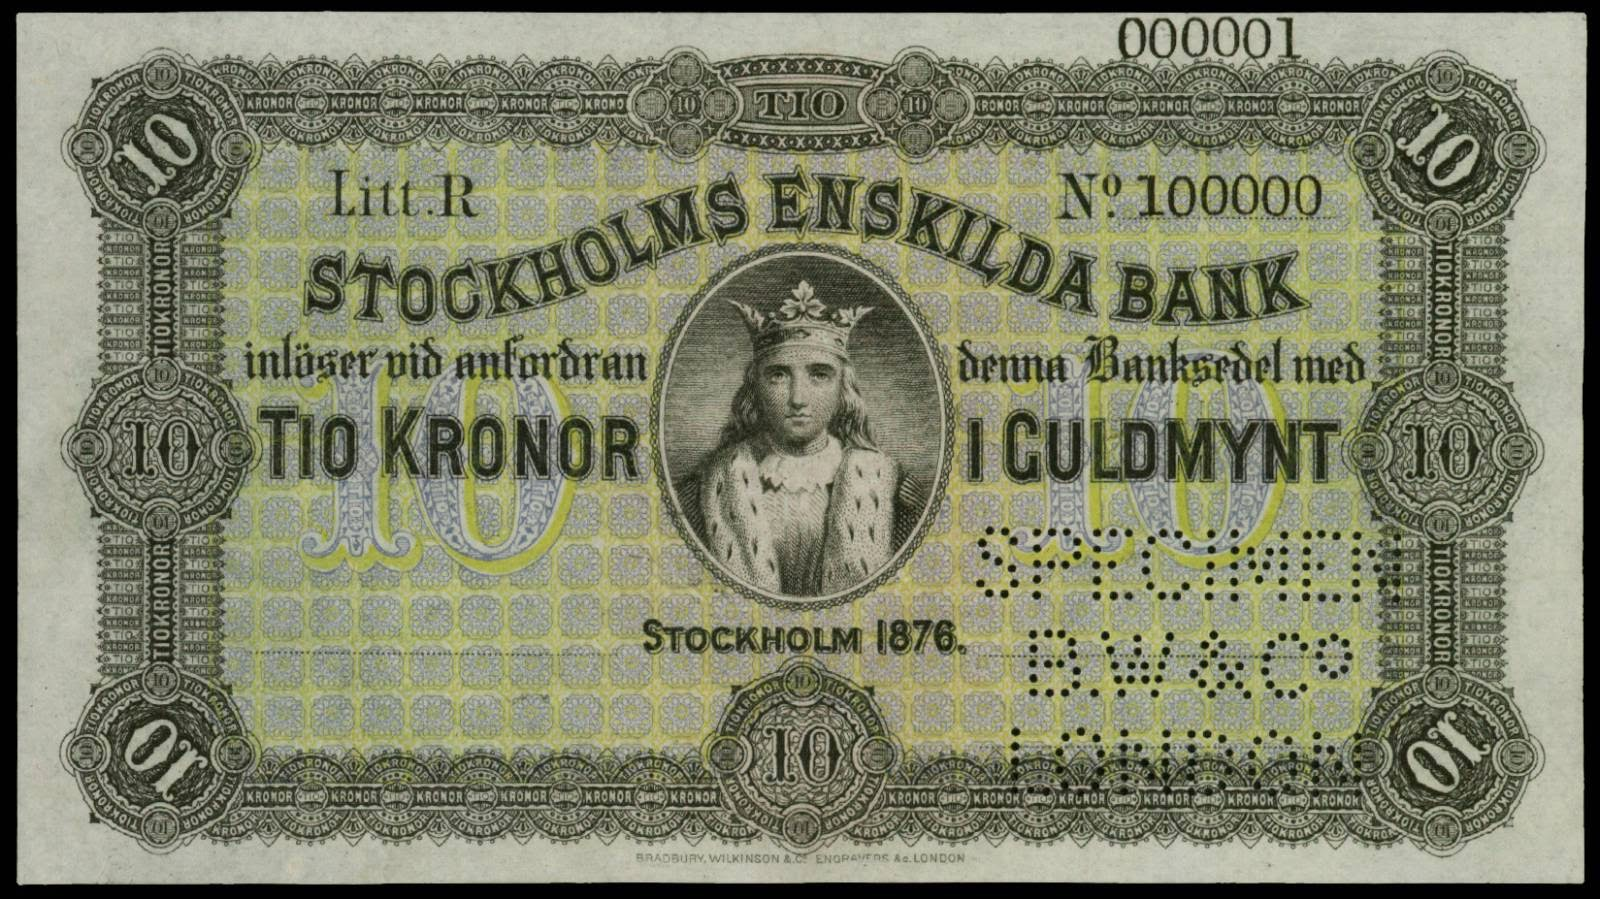
\includegraphics[width=7cm]{PrivateBankNoteStockholmEnskildaBank1876.JPG}
	\caption{\textit{The private bank 'Stockholms Enskilda Bank'(SEB) issued bearer
	promissory note. It promises to pay 10 crowns to the bearer upon demand in gold. 
	The exchange rate as per the Scandinavian Convention(Sweden, Denmark 27 may 1873, Norway 1 april 1877)\cite{nordic:crown}
	was 1 kilogram gold per 2480 crowns or 1 crown per 0.403g gold\cite{crown:gold}. 
 }}
	\label{fig:seb:promissory:note}
\end{figure}

By the late 19th century almost all major currencies was under the gold standard as seen in table \ref{tab:gold:standard}.

\begin{table}[!htb]
	\begin{tabular}{lllll}
		Nation & Currency & Period & Years \\
		France & Franc & 1814-1914 & 100 \\
		Netherlands & Guilder & 1816-1914 & 98 \\
		G.Britain & P. Sterling & 1821-1914 & 93 \\
		Switzerland & Franc & 1850-1936 & 86 \\
		Belgium & Franc & 1832-1914 & 82 \\
		Sweden & Kronor & 1873-1931 & 58 \\
		Germany & Mark & 1875-1914 & 39 \\
		Italy & Lira & 1883-1914 & 31 \\   
	\end{tabular}

	\caption{\textit{ Major European nations periods under the gold standard
			as composed by Ferdinand Lips\cite{lips:gold:wars} from 1975 Pickís Currency Yearbook data.
	}}
	\label{tab:gold:standard}
\end{table}

\subsection{Bank runs}

The introduction of the promissory note solved the two previously mentioned problems but also 
introduced trust.\footnote{Note that this a much wider problem than for only promissory notes. This trust model is what makes banks in the first place.} 

Although the gold deposits could be regularly audited by a third party there is little to no guarantee that the bank in question wouldn't issue more notes than gold it holds in reserve. Banks utilizing this sort of practice could go on for a very long time before getting caught. Consider a bank that issue twice as many notes as it holds gold in reserve. It would require 50\% of it's notes to be demanded before the bank would default.  
  
There has been many so called bank runs in history. The public gets suspicious about the bank and the trust disappears - leading to massive withdrawals in a short time span. Even if a bank is technically solvent, having assets tied up in different ventures, they could fail to deliver on the notes promises. This can also be viewed as a negative spiral, people start to withdraw, increasing the risk of default, more people start to withdraw due to the new higher risk. R.H. Patterson elaborates in detail the bank run in Great Britain in 1866 leading to the default of Overend, Gurney and Company and the behavior under panic: 

\begin{displayquote}
	"When a Panic occurs, a much more serious home-drain is produced upon the bank. At such time cheques fall somewhat into disrepute, so that merchants in some cases require payment in cash. The public also, to some extent, take to hoarding[...]. But a very large part of the drain upon the Bank of England in the form of hoarding ,[...],is made by other banks: for these banks being liable to unusual demands on the part of their customers, have to keep in hand a larger stock of money than usual"\cite{patterson:monetary:drains}
\end{displayquote}

Overall most larger institutions stayed solvent and bank runs is more an exception than a rule during this time period. Since all major currencies were denominated in gold the threshold for global trade sank. During the gold standard era the economy boomed with trade and is often known under the French term 'La Belle Epoque' or 'Beautiful era'. 

\onecolumn

\section{Elasticity of money}

It all came crashing down with the outbreak of the first world war. Nations central banks began to issue more notes than gold in reserve to fund the war effort. It effectively ended the gold standard and countries not affected by the war followed shortly after.

As response the Great Depression U.S President Franklin Roosevelt issued Executive order 6102 confiscating all gold coins, bullion and certificates and banned trade in gold\cite{roosevelt:6102}. The U.S Dollar was devalued the following year from \$20.67 per troy ounce to \$35 under the Gold Reserve Act\cite{gold:reserve:act} to enable spending their way out of recession. 

A new economic era began following ideas of Maynard Keynes of economic interventionism and monetary policies set to aid growth. Keynes rebutted the classical idea that 'supply creates its own demand' and that aggregated demand and aggregated supply may get stuck in an equilibrium with high unemployment\cite{keynes:general:theory}. This would motivate government intervention to increase the aggregated demand. While demand can be altered by a government in multiple ways the far most effective one was altering the money supply\footnote{The increased supply can be used directly by government but is usually used by lowering the funds rate, increasing investments and thus demand. Quantitative easing is another term describing this }. Although the dollar was still technically redeemable for gold the elastic money supply made it possible to steer the economy by means of monetary policy. 

The dollar was re-pegged multiple times between 1968-1971 as part of the Nixon chock\cite{bordo:bretton:woods}. In 1971 Nixon ended the Bretton Woods agreement\cite{bordo:bretton:woods}, the international agreement of exchange rates between currencies, rendering the dollar and all currencies pegged to the Dollar true fiat currencies. After the initial shock the free floating currencies failed to keep pace with gold due to money supply increase causing inflation(Se figure \ref{fig:gold:price:major:currency}).

\begin{figure}[!htb]
	\centering
	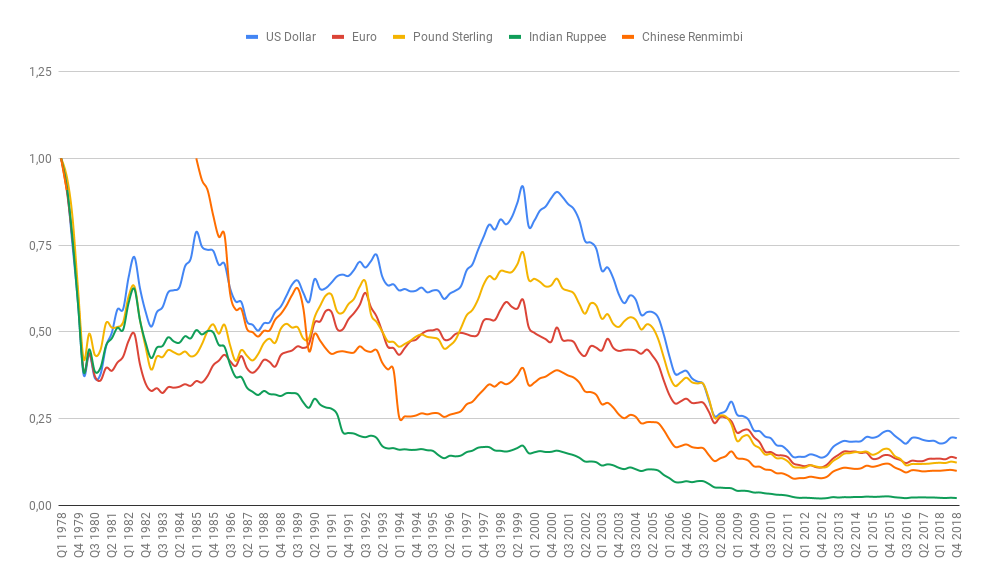
\includegraphics[width=16cm]{gold-price.png}
	\caption{\textit{The relation of major currencies against its value in gold since the end of the Bretton Woods agreement to
			today. The graph is composed with data from the World Gold Council\cite{world:gold:council}. 
	}}
	\label{fig:gold:price:major:currency}
\end{figure}


\twocolumn

\begin{table}[!htb]
	\begin{tabular}{llllll}
		Nation & Currency & Period & Highest monthly Inf. & Avg. daily Inf. & Type of index\\
		Hungary & Pengő & Aug. 1945 - Jul. 1946 & $ 4.19 × 10^{16}\% $ & 207\% & Consumer \\
		Zimbabwe & Dollar & Mar.2007 - Mid-Nov.2008 & $7.96 × 10^{10}\%$ & 98.0\% & Implied Exchange \\
		Yugoslavia & Dinar & 3 Apr.1992 - Jan.1994 & 313,000,000\% & 64.6\% & Consumer \\
		Germany & Papiermark & Aug. 1922 - Dec.1923 & 29,500\% & 20.9\% & Wholesale \\
		China & Yuan & Oct.1947 - Mid-May.1949 & 5,070\% & 14.1\% &	Wholesale \\
		Venezuela(§) & Bolívar & Jan. 2018 - ongoing & - & 4.1\% & - \\ 

	\end{tabular}
	\captionsetup{width=11cm}
	\caption{\textit{ Hyperinflation of selected fiat currencies. From the Hanke-Krus Hyperinflation Table \cite{hanke:krus:hyperinflation:table}. §The Venezuela numbers are only a projection by the International Monetary Fund
			and the dates and rate will most likely change with more accurate data\cite{hanke:hyperinflation} and when the inflationary period is over.
	}}
	\label{tab:inflation}
\end{table}

\subsection{Hyperinflation}

The major currencies seen in figure \ref{fig:gold:price:major:currency} is very far from worst in their ability to hold value. Fiat currencies are highly dependent on it's authority and their willingness to increase the money supply and history supplies us with some catastrophes as seen in table \ref{tab:inflation}.

During the last 250 years hyperinflation\footnote{There is no official definition of what constitutes hyper inflation but a rule of thumb seem to be over 50\% annual inflation.} have occured at least 54 times\cite{hanke:krus:hyperinflation:table}\cite{hanke:hyperinflation}. Many countries going through multiple inflationary periods, e.g. China 43-45, 47-49 and Georgia 92, 93-94. Hyperinflation devastates all savings and effectually letting savings subsidize the newly printed currency. The inflation narrows the time horizon of trade, since capital will go worthless in a short while, making it very difficult to formalize any long term investment or running a normal economy. 

\section{Trust}

The economic system built upon fiat currencies are based on the trust in the issuing body not to increase the money supply excessively. It's almost been common knowledge that value is lost in currencies, moving money away from currency and bonds into stock and real estate. Modern currencies have been decoupled from the underlying reasons of its nascence( see section \ref{sec:characteristics:money}) leading up to the failures of 08 coinciding with Nakamoto's publication completing full circle.

\newpage
\noindent
\vspace{6cm}

\subsection{Relevancy}
In many ways it helps to think of bitcoin as both a bearer instrument and as a monetary policy and how the system is designed as such. This section is an incomplete view on it's own and for further reading these recommendations are good starting points: 

\begin{itemize}
	\item Nick Szabo's blog Enumerated and above cited Shelling out\cite{szabo:shelling:out}.
	\item Saifedean Ammous's The bitcoin standard.\cite{ammous:bitcoin:standard}
	\item Waren Weber's paper A bitcoin standard.\cite{weber:bitcoin:standard}
\end{itemize}
	
	\clearpage
	
	\label{chapter:bitcoin}
	\chapter{The Bitcoin Network}
	\label{sec:bitcoin}

Bitcoin is a peer-to-peer electronic cash system without any trusted third party and was described by Satoshi Nakamoto in Oktober 2008\cite{nakamoto:bitcoin}. The name Bitcoin refers to both the operating network of nodes and the system's native currency. The network and protocol is usually refereed with a large B, Bitcoin, and the currency with a small b, bitcoin.\footnote{While it's convention to not capitalize currencies in the English language, it's not been widely followed in mainstream or semi-mainstream outlets. Also the plural form of currencies is equivalent to the singular. The convention will be followed in this report.}

\section{Digital Signatures}

Part of the solution is provided by one way asymmetric encryption utilizing the \texttt{secp256k1} elliptic curve. Asymmetric encryption or public-key encryption essentially boils down to the ability to derive a public key from a private key without the ability to derive the private key from the public key and the ability to prove ownership of a private key through signatures without disclosing the private key. Ownership of bitcoin is proved by signing a previous transaction output payable to the public key derived bitcoin address\footnote{A bitcoin address is derived from the public key by hashing the public key with both \texttt{SHA256} and \texttt{RIPEMD160}}. 

\begin{figure}[!htb]
	\hspace*{-2cm} 
	\centering
	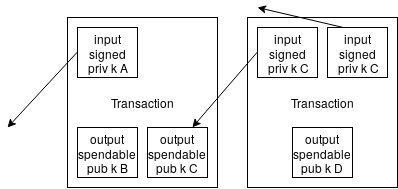
\includegraphics[width=8cm]{transaction.png}
	\caption{\textit{A simplified illustration of two transactions. 
	}}
	\label{fig:merkle:tree}
	\hspace*{2mm} 	
\end{figure}

Bitcoin is essentially a long ledger of inputs and outputs. Note that the whole output must be spent in the same transaction and usually there is an output leading back to an address the spender controls with the 'change'. The sum of all the inputs and the sum of all the outputs usually does not line up, the differential is the implicit miners fee the miner receives if the transaction is included in a block. 

\section{The Double-Spending problem}

While digital signatures are able prove ownership of bitcoin. There is nothing to stop the owner of an amount of bitcoin to sign multiple transactions spending the same transaction output. This is called the double-spending problem which is a variation of the more general Byzantine's General Problem.

Bitcoin solves this by using a data structure composite of a chain of blocks as seen in figure \ref{fig:blockchain}.

\begin{figure}[!htb]
	\hspace*{-2cm} 
	\centering
	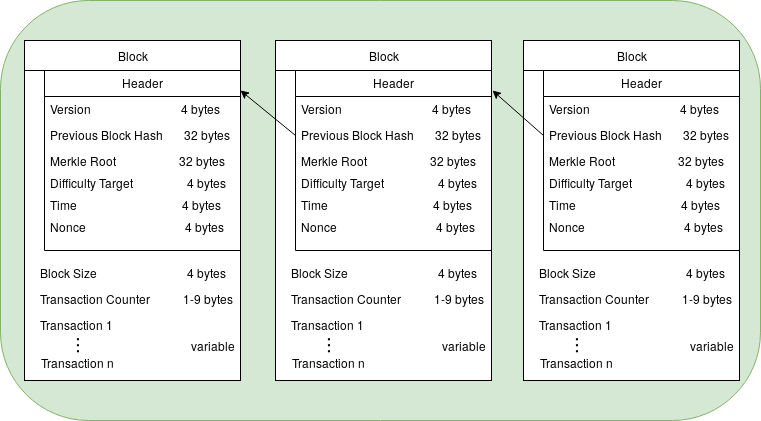
\includegraphics[width=10cm]{blockchain.png}
	\caption{\textit{The blockchain. 
	}}
	\label{fig:blockchain}
	\hspace{2mm} 
\end{figure}

The blocks are chained through the hash of the previous block's header. A block is only valid if the hash is lower than an number imposed by the difficulty target. The hash is deterministic but for all intents and purposes it is random and to find a valid hash one simply hashes the header until a valid hash is found. This process is known as \textbf{mining}. The difficulty target adjusts every 2015th\footnote{This is off by one bug, 2016 blocks is two weeks} block\cite{repository:bitcoin} and forces the average time for a block to be mined to always be ten minutes. This sort of design is known as \textit{Proof-of-Work} and bitcoin differentiate from previous implementations with the difficulty adjustment\cite{back:hashcash}\footnote{Bitcoin uses the dubble \texttt{SHA256} hash, it is essentially the same as hashcash in the cost function being non-interactive, publicly auditable, trapdoor-free and unbounded probabilistic cost\cite{back:hashcash}.}.

\subsection{Merkle Tree}

\begin{figure}[!htb]
	
	\centering
	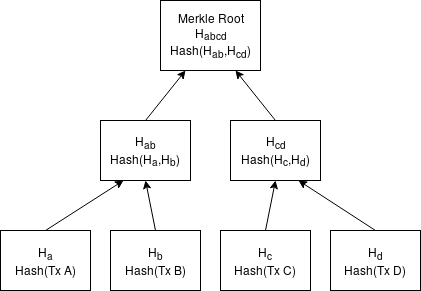
\includegraphics[width=8cm]{merkle.png}
	\caption{\textit{A merkle tree. 
	}}
	\label{fig:merkle:tree}
	
\end{figure}

The content in the block header is effectively unchangeable since a change would make the chain of hash invalid. The transactions are not in the header but are still immutable by the use of a Merkle tree(see fig \ref{fig:merkle:tree}). A Merkle tree is a tree in which the parent is the hash of its two children. The root hash of the tree is included in the header and if any transaction were to change that would cause the root hash to change rendering each transaction immutable by implication. Bitcoin uses the dubble \texttt{SHA256} as the merkle tree hash function.

\subsection{Incentive}

The miners are incentivized by receiving the transaction fees from the transactions included in its block as well as a subsidy. The subsidy is on the form a coinbase transacion which has only outputs, this is how new bitcoin is minted. Every fourth year the subsidy halves and by 2140 will be zero. The miner must follow the consensus rules and mined blocks not following the rules will not be propagated through the network causing the miner to loose out on the block reward. A miner controlling more than 50\% of the hashing power could technically double-spend transactions by mining blocks on an own chain without publishing them and spending on the other chain and then publish the own longer chain. A huge problem with such an attack is that the confidence of the network would decrease causing the value of the 'stolen' bitcoin to be close the worthless and still owning a lot of specialized hashing hardware worthless without the network. In a sense such an attack would cause mutual destruction for both the network and the attacker. 

\section{Script}

Transactions utilize a forth-like polish-notation stack based execution scripting language\cite{antonopoulos:mastering:bitcoin}. Each transaction output consist of a locking script\footnote{Also refereed to as scriptPubKey. Locking script is a broader term and technically scriptPubKey scripts $ \subseteq $ locking scripts.}. In order to spend a valid unlocking script must be provided in the input to the spending transaction that solves the locking script\footnote{scriptSig, witness $\subseteq $ unlocking scripts.}. Validation is performed by executing the unlocking script and locking script sequentially as seen in figure \ref{fig:simple:script}. 

\begin{figure}[!hbt]
	
	\begin{lstlisting}
 <@\texttt{\textcolor{red}{OP\_1}}@>   <@\texttt{\textcolor{green}{OP\_2 OP\_ADD OP\_3 OP\_EQUAL}}@>
<@\texttt{\textcolor{red}{unlock}}@>           <@\texttt{\textcolor{green}{lock}}@>
	\end{lstlisting}
	
	\caption{\textit{ A simple predicate. Evaluated from left to right (1 2 +) -> 3 and
			(3 3 =) -> true. This lock script can obviously be solved by anyone and is thus not used.
	}}
	\label{fig:simple:script}
\end{figure}

The two scripts essentially forms a predicate. If the predicate is true the transaction is true, Nakamoto considered naming the language predicate but went with script to be more inclusive to a broader audience\cite{nakamoto:predicate}.

\subsection{Pay to Public Key Hash}

The Pay-to-Public-key-hash or P2PKH for short was the standard script for a long time. It allows only the owner of 
the private key to the public key to spend the output.


\begin{figure}[!hbt]
	
	\begin{lstlisting}
<@\texttt{\textcolor{red}{<Sig><Pub\_Key>}}@>   
   <@\texttt{\textcolor{red}{unlock}}@>
   
<@\texttt{\textcolor{green}{OP\_DUP OP\_HASH160 <Pub\_Key\_Hash> OP\_EQUALVERIFY OP\_CHECKSIG}}@>
   <@\texttt{\textcolor{green}{lock}}@>
	\end{lstlisting}
	
	\caption{\textit{ The P2PKH locking and unlocking scripts.
	}}
	\label{fig:P2PKH}
\end{figure}

The P2PKH pushed the signature produced by the private key and the public key to the stack. The public key get duplicated and one of them get hashed. The \texttt{OP\_HASH160} is a double hash and first hashes the key with \texttt{SHA256} and then \texttt{RIPEMD160}. This is done to hide the public key until expenditure, which is useful if, for example, the ECDSA would break and private keys could be reversed. The combination of these two hashes makes it way harder to break. In the early days of the network this obfuscation technique wasn't used, for example the first transaction between Nakamoto and Finney didn't\cite{nakamoto:finney:tx}.
The \texttt{OP\_EQUALVERIFY} pops the two public key hashes and terminates the script with false if they are unequal.
The \texttt{OP\_CHECKSIG} verifies that the signature is indeed a match with the public key. 
% In the scripting language uses guard clauses than OP\_EQUALVERIFY, OP\_CHECKSIG should this be mentioned?

\subsection{Pay to Script Hash}

The Pay-to-Script-Hash or P2SH is a more flexible transaction than the P2PKH and was introduced with BIP016\cite{bip:0016:p2sh}. It allows the locking script to only be the hash of the redeemable script. If a cumbersome script with many public keys is considered as seen in figure \ref{fig:cumbersome:script}:

\begin{figure}
	
	\begin{lstlisting}
<@\texttt{\textcolor{red}{0 <Sig A> <Sig B>}}@>   
   <@\texttt{\textcolor{red}{unlock}}@>
	
<@\texttt{\textcolor{green}{2 <Pk\_A><Pk\_B><Pk\_C> 3 OP\_CHECKMULTISIG}}@>
   <@\texttt{\textcolor{green}{lock}}@>
	\end{lstlisting}
	
	\caption{\textit{ Showing a multisig transaction which require to signatures out of three to be spent. Note the \texttt{0} in the unlock script, it's there due to a bug with \texttt{OP\_CHECKMULTISIG} which pops an extra item from the stack. If not for the \texttt{0} it would try to pop an empty stack. The dummy value must be a \texttt{0} with BIP 147 compliant node implementations\cite{bip:0147:dummy:zero}.
	}}
	\label{fig:cumbersome:script}
\end{figure} 

This multisig transaction(in figure \ref{fig:cumbersome:script}) could be rewritten as a P2SH by hashing the locking script with \texttt{SHA256} and  \texttt{RIPEMD160} and utilizing it as seen in figure \ref{fig:p2sh}. Note that 'redeem script' refers to the lock script of figure \ref{fig:cumbersome:script} and 'redeem script hash' it's hash.

\begin{figure}[hbt!]
	
	\begin{lstlisting}
<@\texttt{\textcolor{red}{0 <Sig A> <Sig B> <redeem script> }}@>   
   <@\texttt{\textcolor{red}{unlock}}@>
	
<@\texttt{\textcolor{green}{OP\_HASH160 <redeem script hash> OP\_CHECKVERIFY}}@>
   <@\texttt{\textcolor{green}{lock}}@>
	\end{lstlisting}
	
	\caption{\textit{ The P2SH transaction which is essentially equivalent to the multisig in figure \ref{fig:cumbersome:script}
	}}
	\label{fig:p2sh}
\end{figure}

Converting to a P2SH transaction does two things:

\begin{itemize}

	\item It shifts the fee burden from the sender to the recipient. The locking script is shorter, the unlocking script is longer.
	
	\item All unspent UTXOs must be kept in the RAM of the node, shifting the burden does reduces the node RAM load. 
	
\end{itemize}

P2SH also allows the script to be used as an address(see BIP013\cite{bip:0013:p2shaddr}). By simply sending to the script address could fund any type of complex transaction with no added complexity to the sender.

The scripts can be made quite advanced enabling many layers on top of it, transactions is sometimes be referenced to as 'smart contracts'\footnote{First formally defined by Nick Szabo in 1994\cite{szabo:smart:contracts}}.

\begin{figure}[hbt!]
	
	\begin{lstlisting}	
<@\texttt{\textcolor{black}{IF }}@>
  <@\texttt{\textcolor{black}{IF }}@>
    <@\texttt{\textcolor{black}{2 }}@>
  <@\texttt{\textcolor{black}{ELSE }}@>
    <@\texttt{\textcolor{black}{<30 days> CHECKSEQUENCEVERIFY DROP}}@>
    <@\texttt{\textcolor{black}{<Pubkey D> CHECKSIGVERIFY}}@>
    <@\texttt{\textcolor{black}{1}}@>
  <@\texttt{\textcolor{black}{ENDIF }}@>
  <@\texttt{\textcolor{black}{<Pk A><Pk B><Pk C> 3 CHECKMULTISIG}}@>
<@\texttt{\textcolor{black}{ELSE }}@>
  <@\texttt{\textcolor{black}{<90 days> CHECKSEQUENCEVERIFY DROP }}@>
  <@\texttt{\textcolor{black}{<Pubkey D> CHECKSIG }}@>
<@\texttt{\textcolor{black}{ENDIF}}@>

	\end{lstlisting}
	
	\caption{\textit{ A more complex multisig locking script involving timelocks.
	}}
	\label{fig:aantop:multi}
\end{figure}

One example of a more advanced script is this multisignature locking script with timelock by Antonopoulos seen in figure \ref{fig:aantop:multi}\cite{antonopoulos:bitcoin:scripting}. The script consists of three clauses, the clause executed is left to the unlocking script since the condition to \texttt{IF} is the top item on the stack, not the following item. The output could be spent by either clause being triggered:
\begin{itemize}
	\item 2 out 3 of the A, B, C signatures.
	\item 30 days passed, D signature and 1 out of A, B, C signatures.
	\item 90 days passed and D signature.
\end{itemize} 

The Lightning Network utilize many complex transactions and more on this topic in section \ref{sec:lightning:network}.

\section{Network}

The Bitcoin network consists of nodes complying with the consensus protocol. In the beginning only the reference implementation was used but now there are multiple independent implementations\cite{repository:bitcoin}\cite{repository:btcd}\cite{repository:neutrino}. To participate in the consensus protocol, the nodes relay transactions and valid blocks. If the node is a mining node it also tries to find a new block hashing the previous block on the longest chain. If two valid blocks with the same height is received, the node usually work on the first received until the next block is found breaking the tie. 



	
	\clearpage
	
	\label{sec:scaling}
	\chapter{Scaling bitcoin}

There is no secret that the bitcoin blockchain will not be able to scale on its own. When Nakamoto first published the whitepaper on the cryptographic mailing list his first response was in fact that such a solution won't scale very well\cite{donald:scale}. 

Andreas Antonopoulos has drawn similarities between the scaling of bitcoin with the scaling of the internet:

\begin{displayquote}
	"Bitcoin is failing to scale. If we’re really lucky, bitcoin will continue to fail to scale gracefully for 25 years, just like the internet."\cite{antonopoulos:the:internet:of:money}
\end{displayquote}

His quote in many ways are spot on as Usenet used a \textit{Store-and-forward} method for content to reach every server in the network. \textit{Store-and-forward} does not scale very well and is somewhat similar to the base Bitcoin protocol. The internet moved away from \textit{Store-and-forward} to more direct routing and Bitcoin is too, allowing transactions to happen off-chain.

In this chapter the various scaling alternatives will be discussed.

\section{Block Size limit}

In 2010 Nakamoto reduced the block size limit from 32 to 1 Megabyte as part of two commits. The first commit introduces the new \texttt{BLOCK\_SIZE\_LIMIT} constant\cite{nakamoto:commit:1} and the other commit enforcing the blocks to be under the limit\cite{nakamoto:commit:2}. Nakamoto did not give any explanation as to the reason of this limit. As there was only a few transactions per block at this time a limit reduced the worst case scenario for a DoS attacker filling up the blocks with dummy transactions. 

Increasing the amount of transactions would also increase the imposing cost for the ecosystem by forms of bandwidth, processing, storage and the speed by which blocks propagate through the network. By imposing a block limit the cost of operating a node would be kept low allowing more peers to be able to participate in the network. 

% would come at an increased cost for the ecosystem (bandwidth, processing, and storage for relay nodes, as well as an impact on propagation speed of blocks on the network

% TODO: Math example, compare visa 

\section{Increasing block size limit}

There has been many proposals to increase the block size. Including a handful of BIPs:

\begin{itemize}
	
	\item \textbf{BIP 100} allows the miner to vote on the block limit by encoding a proposed value in the coinbase unlocking script. A 75\% supermajority may increase the block size limit every 2016 blocks. Each period change is limited to only increase by 5\% from the previous period.\cite{bip:0100:dynamic:block:size}
	
	\item \textbf{BIP 101} proposes an immediate increase to 8 megabyte blocks and continue to double every second year. In the two year periods the size would increase at a linear pace based on the block timestamp.\cite{bip:0101:increase:block:size}
	
	\item \textbf{BIP 102} is a simple one time increase to 2 megabytes. The BIP would be triggered if 95\% of the latest blocks signaled support for the upgrade.\cite{bip:0102:increase:2mb}
	
	\item \textbf{BIP 103} aims to increase the block size in accordance with the technology. In practice however it increases the block size with 4.4\% every ~97 day, 17.7\% annually. \cite{bip:0103:increase:with:technology}
\end{itemize}

Most of these BIPs are implemented as a hard forks. Older nodes would regard the bigger blocks as being over the limit and thus invalid.
If poorly executed, without a great majority upgrading the software in time, the network would be forked into two networks with diverging transaction histories. 

% need better name for community worker
\subsection{Contentious Hard Forks}

No proposal to increase the block size has yet received enough support to be activated. This has caused some controversy among community members and multiple have attempted to increase the limit by force. 

One of the earliest attempts to increase the block size was when node Bitcoin XT implemented BIP 101 mentioned above. It failed to reach the miner consensus it required to activate. The BIP 101 was then removed and replaced by a 2 megabyte block limit which forked bitcoin into a new network known as bitcoin classic. Mike Hearn, co-creator of Bitcoin XT along with Gavin Andersen, has made his intention clear arguing that the block size must increase for bitcoin to reach any adoption beyond a fringe niche\cite{hearn:classic}. 

\begin{figure}[!htb]
	\hspace*{-0.7cm} 
	\centering
	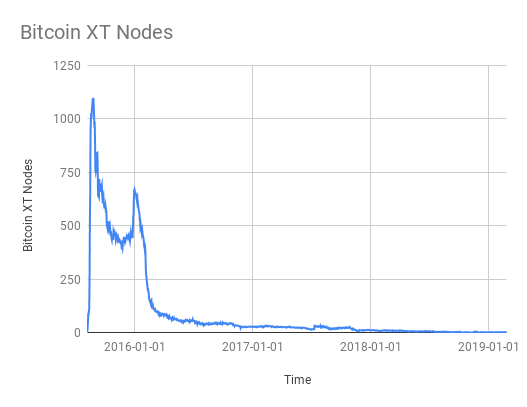
\includegraphics[width=8cm]{external/Bitcoin_XT_Nodes.png}
	\caption{\textit{Historic Bitcoin XT node count. As of 2019-02-25 only 3 nodes are still active. Data retrieved from coin.dance\cite{coin:dance}.}}
	\label{fig:xt_nodes}
	\hspace*{2mm} 	
\end{figure}

As figure \ref{fig:xt_nodes} attests, bitcoin XT and classic failed to receive support and is now dead.

\subsection{The Bitcoin Cash saga}

The failures of Bitcoin Classic was just the beginning of the scaling debate. The proposal of Segregated Witness\cite{bip:0141:segwit} was met with strong opposition as it was considered an overtly complicated and risky upgrade when the block limit could simply be increased. 

Segregated Witness is in a way an increase in block space as it moves the unlocking script(witness) from the transaction to its own structure. Since each transaction takes up less space, more transactions fit in each block. The upgrade also addresses malleability, which many off-chain solutions require, and aligns economics incentives with resource costs\cite{antonopoulos:segregated:witness:align:economic:incentives}. Although its possible to implement Lightning without a malleability fix, it increases its viability\cite{song:lightning:malleability}.

The malleability fix also addresses covert \texttt{ASICBOOST} or Antbleed. Covert \texttt{ASICBOOST} utilizes that part of \texttt{SHA256} may be pre-calculated if the last 16 bits remain the same. The last 16 bytes in the bitcoin header include the last 4 bytes of the Merkle root. By finding two Merkle Roots with the same last 4 bytes, allowing for less computation in finding hashes. To find a matching pair of roots, many roots must on average be tried. The space of viable roots is reduces if the transaction witness isn't malleable\cite{song:asicboost} as the witness can't be manipulated to change the transaction and thus the Merkle root. Gregory Maxwell alluded that \texttt{ASICBOOST} had in fact been implemented in ASIC chips and proposed a fix\cite{maxwell:asicboost:fix}. Bitmain, the largest chip manufacture, made a statement 2 days after addressing the accusation\cite{bitmain:response}. There is no way of ultimately proving if covert \texttt{ASICBOOST} was ever used\footnote{In further conversation with Bitmain representative Nishant Sharma at their headquarters in Beijing in December 2017 he stated that they would never use \texttt{ASICBOOST} of moral reasons. \texttt{ASICBOOST} was not longer viable on Bitcoin at that time, but was on Bitcoin cash and other currencies. He also stated that bitmain had been in negotiation to buy the patent from Timo Hanke and Sergio Demian Lerner and had thus filed a patent for \texttt{ASICBOOST} with the Chinese government. The deal ultimately didn't fell through, and while this information is hearsay at best, the patent sparked many rumors at the time and drove opposition and is one reason for the eventual split.}. 

Segregated Witness When BIP148\cite{bip:148:uasf:segwit}, a \textit{user-activated-soft-fork} scheduled for 22 August 2017 to activate Segregated Witness, was getting traction among nodes, the opposing party(including aforementioned Bitmain) decided to hard fork bitcoin into two by raising the block size limit. The hard fork took place on the first of August 2017 and created Bitcoin Cash.

Bitcoin Cash received significant economic support initially, although significantly below the original chain.


-- Chart over price here --


Although support for Bitcoin Cash has dwindled over the following years, it set a precedence of forks may be utilized. During the second half of 2017 many more forks happened similarly to bitcoin cash.

\subsection{The SegWit2x Compromise}

Most forks are simple copies of bitcoin and may be of little interest here. However SegWit2x carry some historic weight worth noting. 
SegWit2x was originally a compromise 


\section{Removing decentralization}

\section{Side chain}

\section{Off-chain scaling}

(payment channels)

Payment channel networks may be constructed in many different ways, a few distinct proposals has been suggested. Decker and Wattenhofer suggested a \_\_ in which \_\_ however \_\_ \cite{decker:wattenhofer:duplex}.  

\section{Rational for a small blocks}

	
	\clearpage
	
	\chapter{The Lightning Network}
\label{sec:lightning:network}

The \gls{Lightning Network} is a network of micro-payment \gls{channel}s on top of the Bitcoin Network. The network was first conceived and defined in 2014~\cite{poon:dryja:lightning:network}, became viable with the segregated witness upgrade~\cite{bip:0141:segwit} and was activated through a \textit{user-activated-soft-fork} in mid 2017~\cite{bip:148:uasf:segwit}. The upgrade moves(segregates) the unlocking script(witness) from the transaction which fixes transaction malleability since multiple unlocking scripts may be valid for a single locking script. 

The network protocol has been defined~\cite{repository:lightning:rfc} with four independent actors implementing protocol compliant nodes~\cite{repository:lnd, repository:eclair, repository:clightning, repository:lit}.

\section{Payment channels}

The Lightning Network consists of many payment channels between both routing and non-routing \gls{node}s.
A payment channel is essentially a transaction containing funds locked up on the bitcoin network. It requires signatures from both parties to be able to spend the transaction and cease the channel.

Initially each party has a signed transaction splitting the funds to their original committed amount\footnote{In the RFC each channel is funded by only one party so the initial split is always all to one party.}. The parties can then agree on a different balance signing a new transaction invalidating the previous spending transaction essentially allowing for infinite transactions inside the channel without any burden on the bitcoin network.

\subsection{Funding Transaction}

A payment channel is funded by a funding transaction defined in the lightning paper by following steps~\cite{poon:dryja:lightning:network},

\begin{enumerate}
	\item  Create the parent (Funding Transaction)
	\item  Create the children (Commitment Transactions and all spends from the commitment transactions)
	\item  Sign the children
	\item  Exchange the signatures for the children
	\item  Sign the parent
	\item  Exchange the signatures for the parent
	\item  Broadcast the parent on the blockchain
\end{enumerate}

It is critical that the signatures of the spending transaction are exchanged before the funding transaction otherwise the funds could be held hostage by an uncooperative partner\footnote{This is possible with the \texttt{SIGHASH\_NOINPUT} transaction defined in BIP118~\cite{bip:0118:sighash:noinput} which decouples the signature from the specific transaction \gls{hash} of the output. This is not yet activated and only single source funding is currently available}. By exchanging the spending transaction first either party could broadcast it to retrieve the initial funds.

\subsection{Commitment Transaction}

In order for a channel to be useful the creation of a new \gls{commitment transaction}\footnote{It may be easier to think of these types of transaction outputs as smart contracts, as in this context it's the same thing.}, updating the balance, would need to invalidate the previous one. The previous transaction is after all still a valid bitcoin transaction. This creates a problem since each party would benefit from different commitment transactions being broadcast to the network.

The solution is to construct the \gls{commitment transaction} similar to that of a fidelity bond where one party would be penalized if violating the agreement. In this case violation is broadcasting any but the latest commitment transaction. To be able to ascribe blame to the violating party the commitment transactions for the same channel state must be unique as otherwise one would not know which party broadcast the transaction to the network. Only uniqueness is however not enough since there is no way to enforce the penalty for violation.

The enforcement is possible if revocation is built into the commitment transaction, where the other party could revoke a faulty broadcast. This became possible with the addition of relative block maturity introduced with BIP68(see section \ref{sec:rlt}). The commitment transaction has two outputs, one is the other party's funds spendable immediately. The other output has two redeemable paths. Either,

\begin{enumerate}
	\item The broadcasting party can spend the funds after a defined relative block time has passed. Essentially leaving time window for dispute for the violated party to enforce the penalty(Revocable delivery).
	\item The non broadcasting party can refute that the commitment transaction is not last signed and spend the output as penalty.
\end{enumerate}

Remember that the commitment transactions is reversed for the other party. This type of output which enable revocation is called a Revocable Sequence Maturity Contract(\gls{RSMC}).

\begin{figure}[!htb]
			\hspace*{-0.8cm} 
	\centering
	\includegraphics[width=8.5cm]{images/RSMC.png}
	\caption{\textit{Commitment transactions. 
	}}
	\label{fig:commitment:tx}
			\hspace*{2mm} 
\end{figure}

\subsection{Revocation of old commitment transaction}

In order to update the channel balance a new pair of commitment transactions is created. The previous commitment transactions is invalidated by both signing a Breach Remedy Transaction(\gls{BRT}) spending from their own previous \gls{commitment transaction}s \gls{RSMC} output and handing it over to the other party. If a previous commitment transaction were to be broadcast the BRT would take precedence since the revocable delivery takes a certain amount of time before it is valid. The Breach Remedy Transaction will send all funds to the non faulty party, this is the penalty for violating the contract.

It is necessary for each party to monitor the \gls{blockchain} for old commitment transactions and to broadcast the \gls{BRT} in case it happens. If the BRT is not broadcast in the designated time the revocable delivery output of the previous commitment transaction will become valid and may be spent, settling the incorrect channel balance is settled and valid on the blockchain.

\subsection{Alice and Bob opens a channel}

Alice and Bob wants to open a channel. They agree on funding the channel with \textbf{0.5\bitcoin} each. They construct a funding transaction $F$ which require both Alice and Bobs signatures to be spent. Alice constructs a $CT_{A1}$ with two outputs $RSMC_{A1}$ and $SO_{B1}$ and similarly Bob constructs $CT_{B1}$ with outputs $RSMC_{B1}$ and $SO_{A1}$. Alice signs $CT_{B1}$ and Bob signs $CT_{A1}$\footnote{A note on notation - The lowered A,B indicates whether the output is spendable by Alice or Bob. The number denote the channel state the output corresponds to. SO stands for Spendable Output.}. Alice and Bob exchange signatures for $F$ and either of them broadcast $F$.

Alice wants to buy a cookie from Bob for \textbf{0.2\bitcoin} and Bob agrees to sell. They each constructs new \gls{commitment transaction}s $CT_{A2}$, $CT_{B2}$, each with new $RSMC_{A2}$, $RSMC_{B2}$ and $SO_{B2}$, $SO_{A2}$ that reflects the new balance \textbf{0.7\bitcoin} to Bob and \textbf{0.3\bitcoin} to Alice without signing them. Before Bob can hand Alice the cookie the old $CT_{A1}$, $CT_{B1}$ is invalidated by Alice signing a $BRT_{B1}$ spending from $RSMC_{A1}$. Although Bob has nothing to gain by broadcasting $CT_{B1}$ as he would net \textbf{0.2\bitcoin} less - Bob signs $BRT_{A1}$ spending from $RSMC_{B1}$. Alice signs $CT_{B2}$ and Bob signs $CT_{A2}$. The channel balance is updated.

If Alice tries to undo the cookie purchase by broadcasting $CT_{A1}$ giving \textbf{0.5\bitcoin} each. Bob simply broadcasts the $BRT_{B1}$ spending from Alice's share of the $CT_{A1}$ and Bob receives \textbf{1\bitcoin} and Alice \textbf{0\bitcoin}. 

As long as the channel is open Alice and Bob may settle any imbalances between them with a new commitment transaction. 

\begin{figure}[!htb]
		\hspace*{-1.2cm} 
	\centering
	\includegraphics[width=9cm]{images/RSMC_flow.png}
	\caption{\textit{Showing the channel balance state between Alice and Bob after the second Commitment transaction has been made. 
	}}
	\label{fig:rsmc_second_commitment}
		\hspace*{2mm} 
\end{figure}

\subsection{Contracts and implementation}
\label{sec:hdw}
Signing and sending $\gls{BRT}$s is unnecessarily inefficient if a HD wallet is used to generate keys\cite{bip:0032:hd:wallet}. HD wallets have a master key which can derive new keys in a tree structure. Each key in the tree can derive its children and no child can derive its parent. This works both for the public and the private keys independent of each other. A new key is used for each $CT$ and if that is deep in the tree, say a millionth layer down, and can simply be disclosed to the other party whenever the $CT$ is invalidated. The public master key may be shared with the other party so all public keys can be derived for transaction construction. With each new invalidated $CT$ the previous $CT$'s parent key may be used. So each party only needs to store the latest disclosed key as the other child keys can be derived from it.

\begin{figure}[hbt!]
	\centering
	\begin{lstlisting}[
		basicstyle=\small, %or \small or \footnotesize etc.
	]
<@\texttt{\textcolor{black}{OP\_IF}}@>
  <@\texttt{\textcolor{black}{<time> OP\_CHECKSEQUENCEVERIFY OP\_DROP}}@>
  <@\texttt{\textcolor{black}{OP\_HASH160 <A pk> OP\_EQUALVERIFY OP\_CHECKSIG}}@>
<@\texttt{\textcolor{black}{OP\_ELSE}}@>
  <@\texttt{\textcolor{black}{2 <A r pk><B r pk> 2 OP\_CHECKMULTISIGVERIFY}}@>
<@\texttt{\textcolor{black}{OP\_ENDIF}}@>
	\end{lstlisting}
	
	\caption{\textit{ A Revocable Sequence Maturity Contract.
	}}
	\label{fig:RSMC}
\end{figure}

Consider a Revocable Sequence Maturity Contract seen in Figure \ref{fig:RSMC}. It is constructed by Alice and she used Bob's master public key to derive Bob's revocation public key in some prearranged manner. To invalidate the $CT$, Alice need only to disclose the private key corresponding to her revocation public key for Bob to be able to revoke a violation. 

\subsection{Derived revocation address}

The 2 of 2 multi-signature clause paying out to the violated party may be implemented in a denser form by paying to a blinded key neither party control. The private key is then derived from knowledge split between the two parties. When a new $CT$ is created the secret is shared so only the violated party could spend from the revocation clause in case the old $CT$ is broadcast. So hence forth only a revocation pubkey is used to denote a revocation output.

\subsection{Closing channels}

It's possible to close a channel by broadcasting either of the latest $CT$s. However the broadcasting needs to wait the designated time period, losing out on the time value of money. Instead both parties may agree to construct a new Exercise Settlement Transaction($EST$) with direct spendable outputs instead of a $RSMC$ output. Signing the $EST$ would close the channel and allowing both parities immediate access to the funds.

\section{Network wide payments}

By combining channels into a network, a payment could potentially ripple through multiple channels and may allow parties without a direct channel to transact. Such a multi-hop payment would need the same trust-less custodial properties for the routing middle \gls{node}s as between direct channel parties shown above. This is solved by utilizing a Hashed Timelock Contract(\gls{HTLC}) for each of the channels in the route.

\subsection{Hashed Timelock Contract}

A $\gls{HTLC}$ is an extra output added to a $CT$ which enforces a payment from Alice to party Bob if and only if Bob can produce and disclose a preimage R of a \gls{hash} in a designated time period. 

\begin{figure}[hbt!]
	\centering
	\begin{lstlisting}[
	basicstyle=\small, %or \small or \footnotesize etc.
	]
<@\texttt{\textcolor{black}{OP\_IF}}@>
  <@\texttt{\textcolor{black}{OP\_HASH160 <$H_R$> OP\_EQUALVERIFY}}@>
  <@\texttt{\textcolor{black}{2 <A $PK_2$><B $PK_2$> OP\_CHECKMULTISIGVERIFY}}@>  
<@\texttt{\textcolor{black}{OP\_ELSE}}@>
  <@\texttt{\textcolor{black}{<time> OP\_CHECKSEQUENCEVERIFY OP\_DROP}}@>
  <@\texttt{\textcolor{black}{2 <A $PK_1$><B $PK_1$> 2 OP\_CHECKMULTISIGVERIFY}}@>
<@\texttt{\textcolor{black}{OP\_ENDIF}}@>
	\end{lstlisting}
	
	\caption{\textit{ A Hashed Timelock Contract. It's not yet viable for payments in this state.
	}}
	\label{fig:HTLC}
\end{figure}

A $HTLC$ can be seen in Figure \ref{fig:HTLC} and contains two validation paths. 

\begin{enumerate}
	\item If Bob has the knowledge of R that produces $H_{R}$ he can validate the first path. (Execution)
	\item If Bob fails to prove knowledge of preimage R, Alice may validate the second path after the designated time period has passed. (Timeout)
\end{enumerate}

\subsection{Revocation of HTLCs}

$\gls{HTLC}$s have a similar problem as with direct payment channels, if an old $CT$ is broadcast both validation paths may be valid. In the same manner as before, the $HTLC$ is made revocable by the construction of two different contracts for each party $HTLC_{A1}$ and $HTLC_{B1}$. So here again the possibility to ascribe blame exists. Adding revocable paths to $HTLC_{A1}$ and $HTCL_{B1}$ is necessary\footnote{It's necessary to include this path as an uncooperative party may never broadcast the execution/timeout transaction in which revocation is possible.} but not enough since the execution path is also valid. A period for dispute must still be had as the disclosure may be correct but may be from an old commitment transaction. The same is true for the timeout path as Bob may not have knowledge of $R$ in an old commitment transaction.   

Instead the timeout / execution path to oneself is spent into new transactions with a dispute period and ability for the other party to revoke an incorrect broadcast. 

\begin{figure}[hbt!]

	\centering

	\begin{lstlisting}[
	basicstyle=\small, %or \small or \footnotesize etc.
	linewidth=10cm
	]
<@\texttt{\textcolor{black}{OP\_DUP OP\_HASH160 <$H_{RPK}$> OP\_EQUAL}}@>
<@\texttt{\textcolor{black}{OP\_IF}}@>
  <@\texttt{\textcolor{black}{OP\_CHECKSIG}}@>
<@\texttt{\textcolor{black}{OP\_ELSE}}@>
  <@\texttt{\textcolor{black}{<$PK_{B}$> OP\_SWAP OP\_SIZE 32 OP\_EQUAL}}@>
  <@\texttt{\textcolor{black}{OP\_NOTIF}}@>
    <@\texttt{\textcolor{black}{OP\_DROP 2 OP\_SWAP <$PK_{A}$> 2 OP\_CHECKMULTISIG}}@>  
  <@\texttt{\textcolor{black}{OP\_ELSE}}@> 
    <@\texttt{\textcolor{black}{OP\_HASH160 <$R_{preimage}$> OP\_EQUALVERIFY}}@> 
  <@\texttt{\textcolor{black}{OP\_ENDIF}}@>
<@\texttt{\textcolor{black}{OP\_ENDIF}}@>
	\end{lstlisting}
	
	\caption{\textit{ The $HTLC_{A1}$ as offered by Alice
	}}
	\label{fig:alice:HTLC}
\end{figure}

The $HTLC_{A1}$ seen in Figure \ref{fig:alice:HTLC} can only be broadcast by Alice and contains three validation paths:

\begin{enumerate}
	\item Bob can revoke if it's not the last $CT$ constructing a $\gls{BRT}$ spending the output.
	\item The output is spent by a pre-signed transaction to a new transaction $ST$ with a dispute period.
	\item Bob can disclose knowledge of R and spend the output.
\end{enumerate}

The order of the two last clauses is reversed for Bob's $HTLC_{B1}$ as if Bob can prove knowledge of $R$ the output is spent to a new transaction $ST$ for disputation.

\begin{figure}[hbt!]
	
	\centering
	
	\begin{lstlisting}[
	basicstyle=\small, %or \small or \footnotesize etc.
	linewidth=10cm
	]
<@\texttt{\textcolor{black}{OP\_DUP OP\_HASH160 <$H_{RPK}$> OP\_EQUAL}}@>
<@\texttt{\textcolor{black}{OP\_IF}}@>
  <@\texttt{\textcolor{black}{OP\_CHECKSIG}}@>
<@\texttt{\textcolor{black}{OP\_ELSE}}@>
  <@\texttt{\textcolor{black}{<$PK_{B}$> OP\_SWAP OP\_SIZE 32 OP\_EQUAL}}@>
  <@\texttt{\textcolor{black}{OP\_IF}}@>
    <@\texttt{\textcolor{black}{OP\_HASH160 <$R_{preimage}$> OP\_EQUALVERIFY}}@> 
    <@\texttt{\textcolor{black}{OP\_DROP 2 OP\_SWAP <$PK_{A}$> 2 OP\_CHECKMULTISIG}}@>  
  <@\texttt{\textcolor{black}{OP\_ELSE}}@> 
    <@\texttt{\textcolor{black}{OP\_DROP <time> OP\_CHECKLOCKTIMEVERIFY OP\_DROP}}@> 	
  <@\texttt{\textcolor{black}{OP\_ENDIF}}@>
<@\texttt{\textcolor{black}{OP\_ENDIF}}@>
	\end{lstlisting}
	
	\caption{\textit{ The $HTLC_{B1}$ as offered by Bob
	}}
	\label{fig:bob:HTLC}
\end{figure}

The $HTLC_{B1}$ seen in Figure \ref{fig:bob:HTLC} thus contain:

\begin{enumerate}
	\item Alice can revoke if it's not the last $CT$ constructing a $BRT$ spending the output.
	\item Bob can prove knowledge of $R$ the output is spent to a new transaction $ST$ with a dispute period.
	\item After the designated time Alice can spend the output.
\end{enumerate}

The new transactions by which both the second clauses spends to are constructed and pre-signed before the $HTLC$s is exchanged simply adds time for revocation as seen for $ST_{B1}$ in Figure \ref{fig:timeout:tx}.

\begin{figure}[hbt!]
	
	\centering
	
	\begin{lstlisting}[
	basicstyle=\small, %or \small or \footnotesize etc.
	linewidth=10cm
	]
<@\texttt{\textcolor{black}{OP\_IF}}@>
  <@\texttt{\textcolor{black}{<$PK_{RA}$>}}@>
<@\texttt{\textcolor{black}{OP\_ELSE}}@>
  <@\texttt{\textcolor{black}{<time> OP\_CHECKSEQUENCEVERIFY OP\_DROP }}@>
  <@\texttt{\textcolor{black}{<$PK_{B}$>}}@>
<@\texttt{\textcolor{black}{OP\_ENDIF}}@>
<@\texttt{\textcolor{black}{OP\_CHECKSIG}}@>
	\end{lstlisting}
	
	\caption{\textit{ Showing the transaction $ST_{B}$ spends to, the keys are reversed for $ST_{A}$.
	}}
	\label{fig:timeout:tx}
\end{figure}

A $HTLC$ is terminated off-chain by creating a new commitment transaction, without $HTLC$ outputs, reflecting the new balance state as both parties knows what would transpire if the transaction was broadcast. In the creation of the new $CT$ both parties disclose both private keys corresponding to the two revocation outputs as a penalty if an old $CT$ was broadcast. Hence most transactions will be kept off chain and only held in case of an uncooperative party.

In this manner Hashed Timelock Contracts may be used without the need for either of the channel parties to trust each other.

Note that key generation and disclosure may be used for $\gls{HTLC}$ in the same manner previously discussed in section \ref{sec:hdw}.

\newpage
\onecolumn

\begin{figure}[!htb]

	\centering
	\includegraphics[width=15cm]{images/flow_htlc.png}

	\caption{\textit{
			Shows the state of transactions after Alice and Bob have agreed to a new \gls{commitment transaction} $CT_{A3}$, $CT_{B3}$. 
			The transactions to the left side can be broadcast by Alice and the ones to the right by Bob. With the signing of the new $CT$s
			Bob and Alice disclose keys for $BRT_{AH1}$, $BRT_{AH2}$, $BRT_{BH1}$, $BRT_{BH2}$ as penalty if an old commitment transaction is broadcast.
		}}
\end{figure}
\newpage
\twocolumn

\section{Multi-hop payments} 

With properly funded channels and Hashed Timelock Contracts in place network wide payments utilizing multiple channels are possible.
The network uses a Gossip protocol\footnote{as per BOLT\#7 routing-gossip in Lightning RFC\cite{repository:lightning:rfc}} where
public channels are broadcast. Each \gls{node} may then find a path through multiple channels and construct a chain of $HTLC$s with decreasing time locks.

Alice wants to pay David but have no direct path to David. She finds a route via Bob and Carol to David as seen in Figure \ref{fig:multihop}.

\begin{figure}[!htb]

	\centering
	\includegraphics[width=7.5cm]{images/multihop.png}

	\caption{\textit{
			Shows a multihop payment from Alice to Dave across three channels $C_{AB}$, $C_{BC}$, $C_{CD}$. It's critical that the $HTLC$s is constructed in the correct order and with decreasing timesteps $TL_{1}$ > $TL_{2}$ > $TL_{3}$.
		}}
	\label{fig:multihop}

\end{figure}

Alice and David agree on size of the payment and David constructs R and shares $H_{R}$ with Alice. Alice then uses $H_{R}$ to construct a $HTLC_{1}$.
After Alice has created $HTLC_{1}$ with $TL_{1}$, Bob is comfortable creating $HTLC_{2}$ with a $TL_{2}$ < $TL_{1}$ as the only way Carol could redeem $HTLC_{2}$ is by disclosing R to Bob. Bob in turn may then disclose R to Alice and redeem $HTLC_{1}$. If the timelocks were improperly set as $TL_{2}$ > $TL_{1}$ the $HTLC_{1}$ may be invalid by the time Carol redeem $HTLC_{2}$ leaving Bob paying Carol but without getting payed by Alice.

\section{Routing fee}

The routing \gls{node}s receive a fee as compensation for displaced channel liquidity, the time value of money and operational cost of bandwidth, computation and electricity. The fee is structured with a base fee $F_{B}$ and a fee $F_{R}$ proportional to satoshis forwarded $AF$. The base fee is always paid independent of payment size while the proportional part is the product of size and fee. The base fee is denominated in microsatoshi (\textbf{μS}) and the proportional in microsatoshi per satoshi forwarded (\textbf{μS / S}). The fee for a payment $P$ is thus:

\[ F_{P} = F_{B} + (AF * F_{R} / 1000000) \]

This fee structure does not discriminate for channel balance and it is difficult to 'discount' transactions that 'balance' the network. Reasons for this is given in Chapter 8.  

	
	\clearpage
	
	\label{sec:evaluation}

	\chapter{Evaluation}

With the eventual growth of the Lightning Network a fee market for channel liquidity will emerge. How routing nodes 

\section{Lightning network as a graph}

The Lightning Network may be modeled as a directional Graph $G$ with vertices representing nodes and edges representing channels. As each channel may have different fees and liquidity in each direction it's useful to represent each channel with two edges. One edge in each direction. 

\begin{figure}[!htb]
	\hspace*{-0.7cm} 
	\centering
	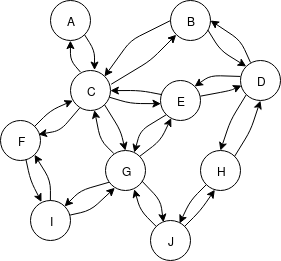
\includegraphics[width=7cm]{images/LN_overview.png}
	\caption{ \textit{A representation of LN as a graph. Each channel is symbolized by two edges.} 
	}
	\label{fig:ln:graph}
	\hspace*{2mm}
\end{figure}

Modeling the network as a graph allows the use of graph theory. Thus routing, concepts of centrality and analytical frameworks may be borrowed from the extensive literature on graphs. The topology of both testnet and mainnet is visualized in Figure \ref{fig:topology}.

\section{Fee as a competitive equilibrium}

It may be useful to view the fee market as existing under normal free market pressures and apply the conventional long run demand and supply curve\cite{boulding:evolutionary:economy} to the fee market. 

\begin{figure}[!htb]
	\hspace*{-0.3cm} 
	\centering
	\includegraphics[width=11cm]{images/equilibrium_sized2.png}
	\caption{ The fee market as viewed according to standard price theory. Both by single pair and all pairs in aggregate. 
		}
		\label{fig:equilibrium}
		\hspace*{2mm} 	
\end{figure}

The demand curve DD' signifies users demand to utilize a shortest path in the lightning network and the supply curve the existing competing paths between s and d. Say there exists a Equilibrium point E by with the market price will move towards. Suppose the average fee price is greater than equilibrium at $F_{1}$ with demand $F_{1}D_{1}$ and supply $F_{1}S_{2}$, and more operators would open a path between s and d driving the curve fee towards E. If it instead lay under the equilibrium at $F_2$ their would be an excess supply $F_{2}S_{1}$ and low demand $F_{2}D_{2}$, making operators loose money by having liquidity locked up on a path not used. Thus leading operators to close channels between s and d, again driving the fee towards E.

The fee market may also be seen in its aggregate, where the axis represents the whole network. Here the drivers might be seen as new routing nodes joining if its a profitable venture or leaving if its a unprofitable one. Here again driving prices towards equilibrium. 

It may be unusual to view demand through the usage of its medium, their is of course a dimension here between payment systems. But there's also a the possibility of streamable payments where the say one's rent might be paid hourly or a documentary per second dependent on the fee price. With a decreased fee these payments becomes more viable driving demand.

The cost of procuring a shortest path between s and d might not be equal for two different routing nodes dependent on already existing paths and set strategies. The viability of a strategy is in essence determined in its ability to be included in shortest paths between nodes.

\section{Fee floor}

The fee price, assuming rational actors, can only fall to a level where the operators are able to sustain their operation. The fees received must compensate for the \textit{time-value-of-money}, the security risk of having liquidity on a connected public node and the operational cost of running and managing the software. Bhatia has proposed a standardized reference rate as Lightning Network Reference Rate(LNRR) similar to LIBOR, OIS and SOFR~\cite{bhatia:time:value}. Operational cost isn't included in LNRR as with managed funds a  operational fee is removed after the returns are calculated. The competition of fees drives down the price until a certain point, a floor, where there is better returns elsewhere. Therefor a the fee has a floor at

\[ F_{floor} = C_{op} + C_{risk-prem} + C_{risk-free-rent} \]

Note that the operational costs are independent of liquidity while the security risk premium and risk-free-returns are dependent.

\subsection{Security Risk premium}

\subsection{Time value of money}


\section{Routing strategies under Game Theory}

There are clearly marked dynamics at play here. Node operator have many different options at their disposal and although all actors may not be rational their behavior should approximate the behavior of maximizing profit. In economic theory optional behaviors as an \textit{agenda field} and the iterable process of finding the maxima as climbing the \textit{maximand hill} with an equilibrium lay at the top~\cite{boulding:evolutionary:economy}. Further each actor's profit depends on every other actor's behavior reasonable to regard it as a Game Theoretic problem. More exactly it resembles a subset of Game Theory similar to that of biological ecosystems first studied by W. D. Hamilton~\cite{hamilton:behavior} and later expanded to a rigorous framework by J.M Smith et al.~\cite{smith:price:logic:animal, smith:evolution:games} as Evolutionary Game Theory (EGT).

In an ecosystem, species survival and propagation in the gene-pool depends on its behavior relative to the population. An aggressive animal may do very well in competition for feed in a population of mostly coy animals. However against a population of mostly aggressive beings it may have to fight most encounters and end up wounded leading to a coy behavior to be preferred. Unsuccessful individuals die off and are removed from the population and subsequently successful individuals prosper and it's genes increases in the population. In Game Theory a Nash equilibrium is an state in which no actor can change strategy and receive a strictly higher payoff~\cite{nash:equilibrium}. In EGT this notion is slightly modified and named Evolutionary Stably Strategy(ESS) which disallows for an actor to change strategy and receive an equal payoff as that would allow for the population to constantly drift between those to strategies. 


Although Lightning nodes doesn't pass on genes, successful strategies are more likely to be copied than unsuccessful ones. Especially if strategies and tool are built as extensions/plugins and made available as open source and freely propagate. Similarly stable points where no node can change strategy and increase profit suggests the viability of the played strategies and hints at the emerging topology. 

To evaluate strategies, the game is divided into five categories.

\begin{enumerate}
	\item \textbf{Fee}, Determine the fee on the outgoing
	\item \textbf{Preferential Attachment}, Determine which nodes to open channels with.
	\item \textbf{Timing}, When to open and close channels.
	\item \textbf{Allocation}, How much capital should be allocated for each channel.
	\item \textbf{Funding}, How much capital is available to the node.
	\item \textbf{Re-balance}, When and how aggressively should a node re-balance its channels. 
\end{enumerate}

Most categories are quite distinct and natural to separate but there is some ambiguity here. Preferential Attachment could very well be considered as the same category but are kept apart to keep the complexity down. Each routing node may then choose a strategy per category, it is sufficient to only consider pure strategies. Mixing of strategies, e.g behaving 'aggressive' 70\% of the time and 'coy' 30\% of the time, is perfectly reasonable to assume. However convergence to a mixture is equivalent to the population mixture of pure strategies. Any equilibrium with only pure strategies could thus be transposed in to a mixed strategy~\cite{easly:kleinberg:network:crowds:markets}. This conveniently reduces the complexity of the simulation without compromising the results. 


It should be noted that profit may not be the only parameter worth maximizing as privacy can be increased with a behavior deviating from a strictly most profitable action.   

does any channel opening algorithm perform better than another and essentially force the network into a scale free hub-spoke network instead of a mesh network?

\newpage
\onecolumn

\begin{figure}[!htb]
	\hspace*{-0.7cm} 
	\centering
	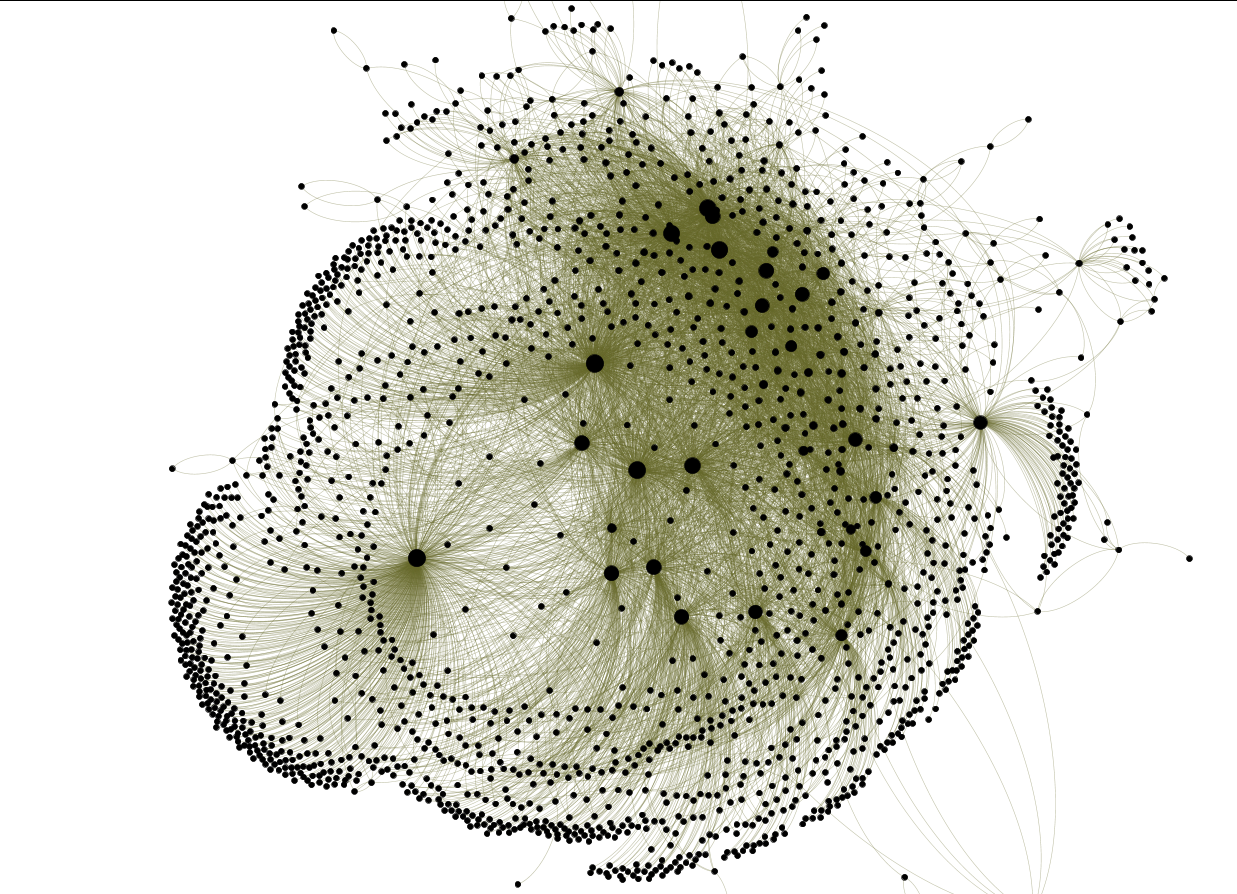
\includegraphics[width=12cm]{graphs/testnet_force.png}
	\vspace*{-0.4cm} 
	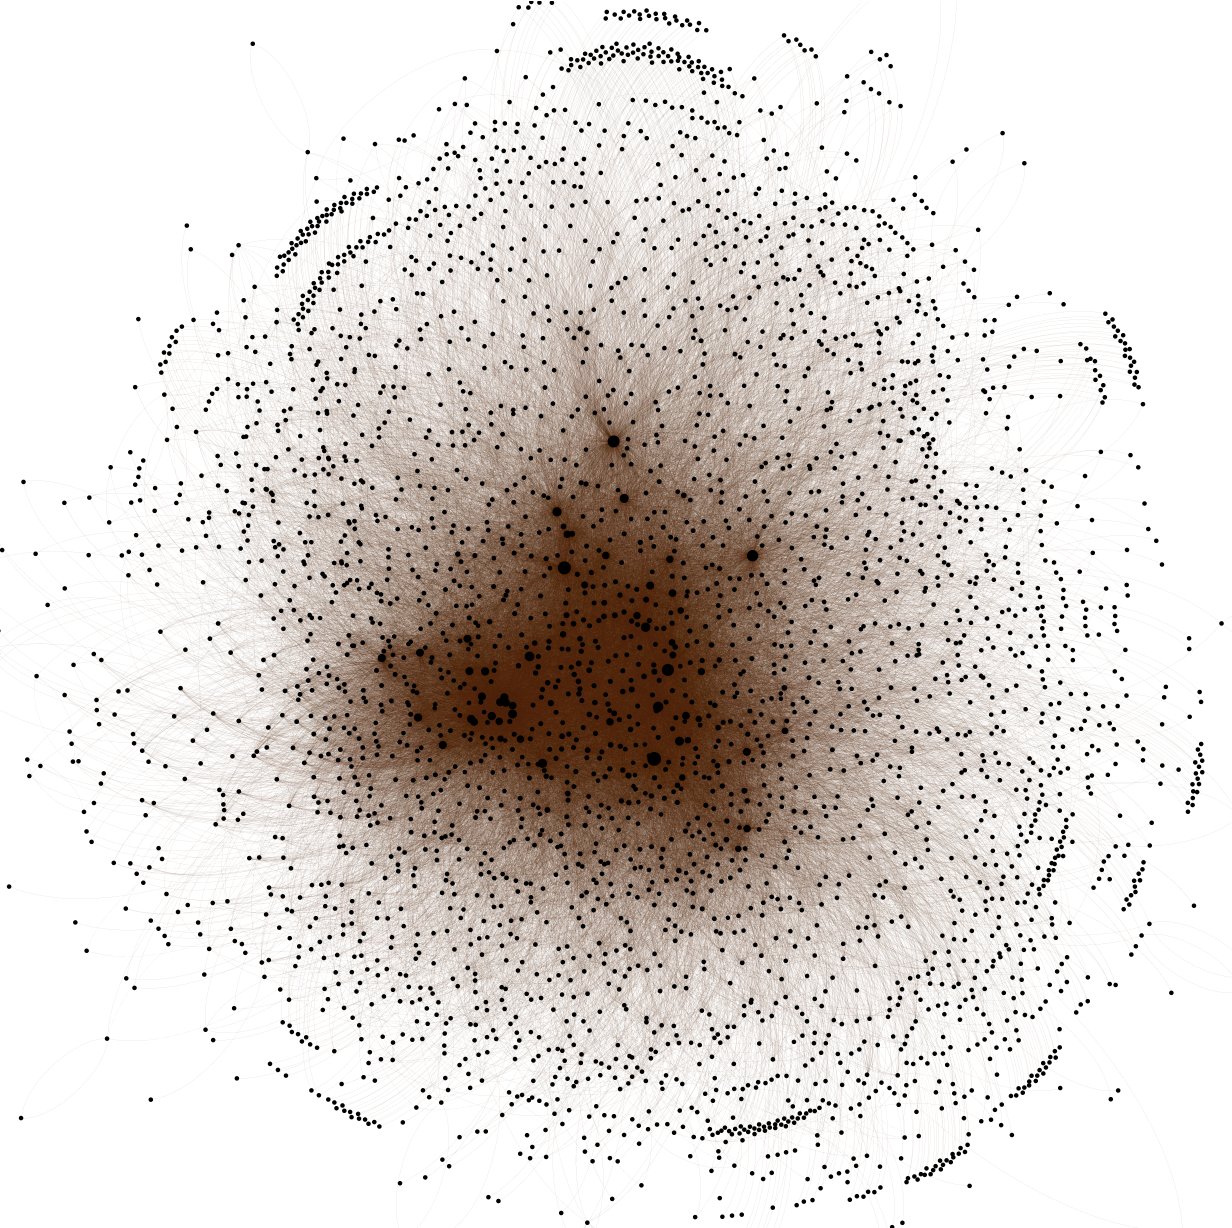
\includegraphics[width=13.6cm]{graphs/mainnet_force3.png}
	\caption{\textit{
			Shows testnet above and mainnet below as of 2019-02-25. Node size corresponds to degree, larger degrees to larger size. Positioning is a mix between Force Atlas and Fruchterman Raingold. Network data retrieved by running a c-lightning node and visualized with Gephi\cite{repository:gephi}.}}
	\label{fig:topology}
	\hspace*{2mm} 	
\end{figure}
\newpage
\twocolumn

\section{Optimal fee price}

To determine the fee price, one could intuitively imagine that and increased fee price would yield higher fees but for less pairs as other paths may become shorter for pairs to route through. So the amount of shortest paths passing through a vertex must be calculated. In 1977 Freeman introduced a measurement named \textit{Betweenness Centrality}\cite{freeman:betweenness:centrality} and defined it as

\[ g(v) = \sum_{s \neq v \neq d}\frac{\sigma_{sd}(v)}{\sigma_{sd}} \]

Where $\sigma_{sd}$ are all shortest paths from s to d and v is vertex. As the fee is determined on an edge basis the definition is altered to regard edges instead of vertices. 

It is possible to determine the optimal fee for an edge if some assumption, of the probability of all pairs transacting and the probability of the size of the transactions, are made. If a uniform probability over all pairs and that the shortest paths are used are assumed the optimal price is given by

\[ x_{opt} \textrm{ is the optimal price } iff \]

\[ f: X \to \mathbb{Z} \textrm{ and } (\forall x \subseteq X)f(x_{opt}) \geqslant f(x) \textrm{ where }\]

\[ f(x) = x\sum_{s \neq e \neq d}\frac{\sigma_{sd}(e(x))}{\sigma_{sd}} \textrm{ and } \]

%\[ \sigma_{sd}(e(x)) =  \begin{cases}
%		n, & \text{if n shortest paths exists} \\
%          & \text{through $e$ with weight x.} \\
%		0, & \text{otherwise}
%	\end{cases} \]

\[ \sigma_{sd}(e(x)) =  \begin{cases}
 & \text{Is the sum of shortest } \\
 & \text{paths between $s$ and $d$} \\
& \text{through $e$ with weight x.} \\

\end{cases} \]


The $\sigma_{sd}$ represents the total amount of shortest paths between $s$ and $d$.
The function $f(x)$ behaves as seen in figure \ref{fig:fee_curve} for a fictitious generated graph. 

\begin{figure}[!htb]

	\centering
	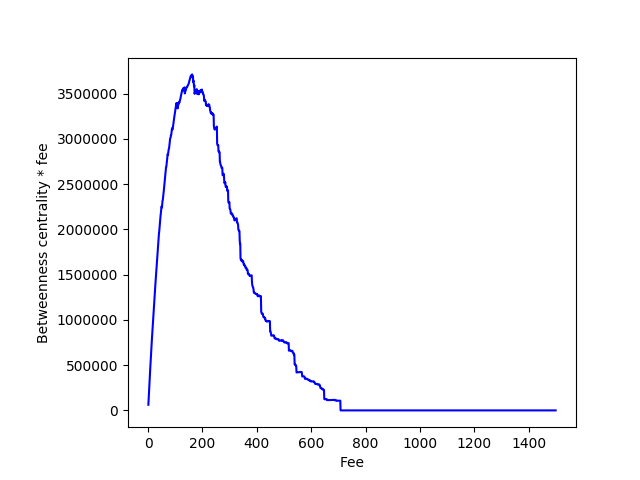
\includegraphics[width=8cm]{images/fee_curve.png}
	\caption{ Shows the betweenness centrality * fee / fee for an edge in a generated graph with 1000 vertices, 5000 edges, uniform weight distribution over 1-1500 and random attachment policy. It holds intuitively as for low fees, many shortest paths passes but procure small overall profits as the fee is small. The profits increases with the increase in fees until a point where the decrease in paths overtakes the increase in fees.
	}
	\label{fig:fee_curve}

\end{figure}

Freeman also defined a centrality measurement for whole graphs, it utilizes the betweenness centrality of every vertex and is thus brutal to calculate in practice for larger graphs. 

Efficient algorithms for edge betweenness centrality have been developed\cite{brandes:betweenness:centrality:algorithm}. Although it is possible to run such an algorithm for each potential fee price to find the optima it would be very slow.
Instead the optimal fee price an for outgoing channel $e$, still holding the assumptions as before, may be calculated by following steps.

\begin{enumerate}
	\item Calculate the shortest path from all-to-all vertices without going through $e$ with either Floyd-Warshall~\cite{bakhtiar:floyd:warshall} or Johnson~\cite{johnson:shortest:path:sparse:network} obtaining table A.
	\item Calculate shortest path from the source of $e$, $V$-to-all explicitly going through $e$ with Dijkstra obtaining table D where $e$ weight set to 0.
	\item Retrieve the difference for all pairs between the all-to-all distance with the all-to-$V$-to-all distance, A[s][d] - (A[s][V] + D[d]). Throw away the negative values and produce a cumulative summation over the differences in a table H.
	\item Select $x_{opt}$ such that \[ \forall x (x H(x)) \leq x_{opt} H(x_{opt}) \]

\end{enumerate} 

Whenever Floyd-Warshall or Johnson should be used depends on the sparseness of G as Floyd-Warshall have a time complexity of

\[ O(V^3) \]

only dependent on vertices whereas Johnson

\[ O(V^2 log(V) + VE ) \]

depends on both edges and vertices. 

\subsection{Cost function}

The fee is in part proportional to the size of the payment, and the aforementioned algorithm is only able to find the optimal price for one payment size.  

 

\section{Topology and Preferential Attachment}

Setting fee price is only one aspect of a routing node, maybe more importantly is that of opening and closing channels.
As the protocol now stands\footnote{Is very plausible that that BIP66 may be activated allowing multi-sourced channels\cite{bip:0118:sighash:noinput}} it only allows for single source funding of channels. There is a non negligible cost to opening channels and it would be very beneficial for a node if other nodes opened channels with it instead of the other way around. This is also a prerequisite to earn profit as otherwise the node may only earn back its own funding. 

Therefor the policies determining by which preferences each node takes into account to open channels is of interest. Further these policies also affects the topology of the network, the average shortest path and robustness in case of node failures.

\subsection{Traditional random models}

Random graphs have been studied extensively, specifically the Erdős–Rényi model\cite{erdos:renyi:random:graphs}. An ER graph is created by denoting a graph $G_{n,N}$ with $n$ vertices and $N$ edges. The edges is then selected randomly from set of ${n \choose 2}$ possible edges. A common approach today is to write $G_{n,p}$ with $p$ being the probability of two vertices having an edge. It's difficult to justify LN behaving as an Erdős–Rényi graph as it allows for isolated points and there is no inherent age bias present. 

Callaway et al.~\cite{callaway:hopcraft:randomly:grown:graphs} added a phase transition to random graphs as to adjust for a supposed age bias. Consider $G_{n,\delta}$ where at first the graph is empty and for each time step a vertex v is added to the $G$ and an edge is selected over $G_v \choose 2$ with a probability $\delta$ until $G$ has $n$ vertices. $G_{n,\delta}$ would have on average $n\delta$ edges and since $n\delta < n$ it only produces sparse graphs. As before this may be difficult to apply to LN as a poorly connected graph would have high average paths and surely many payments would fail. It is however interesting to regard the degree distribution compared to that of Erdős–Rényi as it's exponential given as

\begin{equation}
	p(k) = \dfrac{(2\delta)^k}{(1 + 2\delta)^{k+1}} 
	\label{eq:callaway}
\end{equation}
compared to Erdős–Rényi which is binomial

\begin{equation}
	p(k) = {n-1 \choose k} p^k(1-p)^{n-1-k} 
	\label{eq:erdos:renyi}
\end{equation}

as follows from definition as ${n-1 \choose k}$ are all possible combinations of k edges,  $p^k$ the probability of any combination taking place and $p^k(1-p)^{n-1-k}$ to exclude combinations of larger degree $k$.

Thus adding an age bias causes the characteristics of the degree distribution to change as seen in Figure L.

\begin{figure}[!htb]
		\hspace*{-0.5cm} 
	\centering
	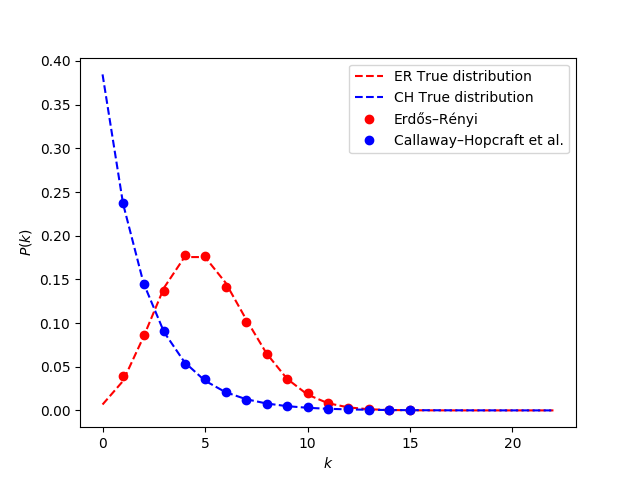
\includegraphics[width=9cm]{images/random_topology_degree_distribution.png}
	\caption{Shows the degree distribution for an Erdős–Rényi graph(\tikzcircle[blue, fill=blue]{2pt}) with n = 10,000, p = 0.0005 and its true distribution given by Equation \ref{eq:erdos:renyi}(\textcolor{blue}{|}) compared to the degree distribution for a Callaway et al. graph(\tikzcircle[red, fill=red]{2pt})  with n = 10,000, $\delta$ = 0.8 and its true distribution given by equation\ref{eq:callaway}(\textcolor{red}{|}).
	}
	\label{fig:fee_curve}
		\hspace*{2mm} 
\end{figure}

A more appropriate random model may be to consider $G_{n,m}$ where each time step $t$ a vertex is added to the graph and is connected with $m$ previous vertices and creates and edges when t < n. The probability of any previous vertex $i$ being selected is thus $p_i = \dfrac{m}{t_i}$. 
As a node may not be viewed as part of LN before edges are made, it's reasonable to assume a node creates edges as part of joining the network.

%[p(k) =  \begin{cases}
%& \prod_{i=1}^{k} 1 - \sum_{j=1}^{n-1} m \dfrac{1}{n^2},~\text{if}~m<k\\
%& 0,~~~~~~~~~~~~~~~~~~~~~~~~~\text{otherwise}

%\end{cases} \]

%\[ \prod_{i=1}^{k} 1 - \sum_{j=1}^{n-1} m \dfrac{1}{n^2} \sim 1 - m^k(\dfrac{1}{2})^k\]

\subsection{Scale free models}

In 1999 Barabási and Albert showed that many networks degree distribution follows a power law and that the distribution was independent from scale, thus scale free\cite{barabasi:albert:emergent:scaling}. Scale free networks follows a degree distribution of

\begin{equation}
	 p(k) \propto k^{-\gamma} 
	\label{eq:scale:free}
\end{equation}

and large network has been shown to follow this model. With notable networks of web hyperlinks having $\gamma_{www} = 2.1\pm 0.1$ and an actor collaboration graph having $\gamma_{actor} = 2.3\pm0.1$. Further suggestions have been made that network have an innate bias, as what has many links is well known and what is well known will receive many links - akin on the \textit{Pareto distribution}("80-20 rule") or the \textit{Matthew Principle}\footnote{As per KJB \texttt{Matthew 13:12 - For whosoever hath, to him shall be given, and he shall have more abundance: but whosoever hath not, from him shall be taken away even that he hath.}~\cite{king:james:bible} }. 
A model was suggested to generate a scale free graph $G_{n, m}$ by starting with a graph with $m$ fully connected vertices, and for each time step adding a new vertex and creating $m$ edges with a bias towards vertices with high degree. The vertex may be said to have a preferred attachment and the probability of a vertex receiving an edge from the new vertex:

\[ \Pi(i) = \dfrac{k_i}{\sum_{j}^{}k_j}  \]

Such a graph follows the scale free property with a $\gamma_{ba}$ = 2.9 and can be seen in Figure \ref{fig:scale_free}
\newpage
\begin{figure}[!htb]
	\hspace*{-0.5cm} 
	\centering
	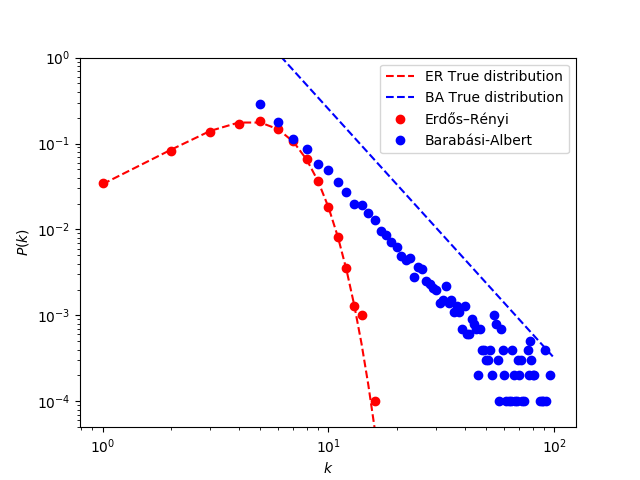
\includegraphics[width=9cm]{images/scale_free_degree_distribution.png}
	\caption{Shows the degree distribution for an Barabási–Albert graph(\tikzcircle[red, fill=red]{2pt}) with n = 10,000, m = 5 and the scale free\ref{eq:scale:free}(\textcolor{red}{|}) with $\gamma$ = 2.9 compared Erdős–Rényi graph(\tikzcircle[blue, fill=blue]{2pt}) with n = 10,000, p = 0.0005 and its true distribution given by Equation \ref{eq:erdos:renyi}(\textcolor{blue}{|}).
	}
	\label{fig:scale_free}
	\hspace*{2mm} 
\end{figure}

%modified barabasi

The actual degree distribution of the lightning network can be seen in Figure \ref{fig:real_network}.

\begin{figure}[!htb]
	\hspace*{-0.5cm} 
	\centering
	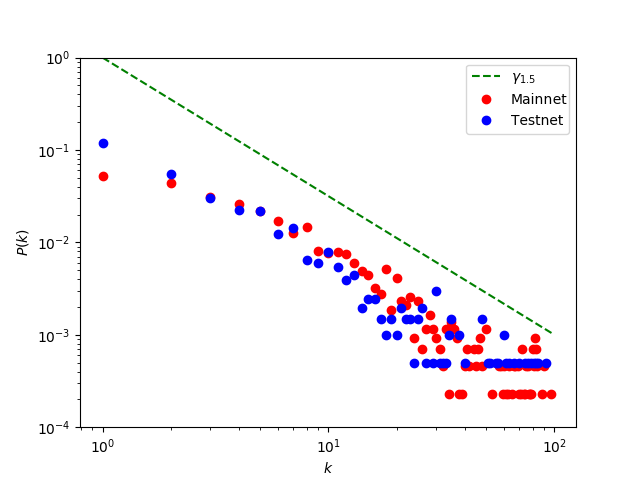
\includegraphics[width=9cm]{images/main-testnet_degree_distribution.png}
	\caption{Shows the degree distribution for both the Mainnet (\tikzcircle[red, fill=red]{2pt}) and Testnet (\tikzcircle[blue, fill=blue]{2pt})
		compared to the scale free function \ref{eq:scale:free}(\textcolor{black}{|}) with $\gamma$ = 1.5. The data is retrieved running a c-lightning node\cite{repository:clightning} on 2019-03-21.
	}
	\label{fig:real_network}
	\hspace*{2mm} 
\end{figure}
% Mainnet 4322 nodes and 21258 edges
% Testnet 2027 nodes, 8712 edges  

It should again be stated that the Lightning Network is still in a very early state of it's development and most of the nodes and transactions over the network are made by enthusiasts trying it out. So the current state of the degree distribution may indicate very little of future states. 

\subsection{Mediation-driven attachment}

Rather than explicitly attaching with a degree bias as with the Barabási-Albert model, Hassan et al.~\cite{hassan:islam:haque:mediation} have suggested a more subtle approach by attaching to a random neighbor of a randomly selected mediator node. Consider a node $i$ which degree $k_i$ and neighbors $1,2,...,k_i$ each having a degree of $k_1, k_2, ... k_{k_i}$ would thus have a probability $\Pi(i) \propto k_i$ and more explicitly:   

\[ \Pi(i) = \dfrac{1}{N} \bigg\lbrack \dfrac{1}{k_1} + \dfrac{1}{k_2} + ... + \dfrac{1}{k_{k_1}} \bigg\rbrack = \dfrac{\sum_{j=1}^{k_i}\dfrac{1}{k_j}}{N} \]

From


\subsection{Connectivity}

\subsection{Fitness models}

Fitness heuristics added bianconi-barabasi~\cite{bianconi:barabasi:fitness:network}.

\[ \Pi(i) = \dfrac{\eta_ik_i}{\sum_{j=1}^{n}n_jk_j}\ \]

\[ \dfrac{\partial k_i}{\partial t} = m \dfrac{\eta_ik_i}{\sum_{j=1}^{n}n_jk_j} \]


\section{Re-balancing channels}

\section{Funding, timing and allocation strategies}

\section{Simulation}

The aforementioned strategies and a simulation environment were implemented in python 3.5 with extensive use of the networkx library. The environment variables and each players chosen strategies can be changed in a higher level meta-language. Each strategy is discussed in detail in Appendix \ref{chapter:strategies} as well how a game may be created and simulated from altering the input file.  


% THE ADJUSTABLE SCALE FREE  http://www.uvm.edu/pdodds/files/papers/others/2002/holme2002a.pdf

% https://webusers.imj-prg.fr/~ricardo.perez-marco/publications/articles/antrouting3.pdf

% https://bitfury.com/content/downloads/whitepaper_flare_an_approach_to_routing_in_lightning_network_7_7_2016.pdf
	
	\clearpage
	
	\label{sec:results}
	\chapter{Results}


(preferential attachment)

(pricing)

(funding)

(open close)

(degree distribution)
(profit distribution)

(re-balance channel)

(combined best strategies)

(is strategy set stable from invasion)

(external pressures, payment pressure, routing / private channels.)
	
	\clearpage
	\label{sec:discussion}
    \chapter{Discussion \& Conclusions}

\section{Complexity}

When the network grow it will eventually become to cumbersome for every node to Floyd-Warshall the whole network as this simulation assumes. Approx. will propably be used. Ant routing tables have been suggested but might be problem with lying about connectedness.

	\clearpage

    \onecolumn
    \newpage
    \addcontentsline{toc}{section}{References}
    \bibliographystyle{plain}
    \bibliography{references.bib}

    \begin{appendices}
%    \chapter*{Routing Fee Protocol Proposal}

Although there is methods to balance channels it would be beneficial if the fee could reflect the state in which the channel is left.

Currently the fee is only proportional to the liquidity used, not the state of the channel.

Suppose there exists a channel between Alice and Bob with 10 million satoshis in it. 
Two payments, $P_{1}$ and $P_{2}$ is routed through the channel from Bob to Alice.
Both use the same amount of liquidity 3,500,000 satoshis each, but the they start from
two different channel positions $B_{1}$ and $B_2$.

\begin{figure}[!htb]
	\hspace*{-0.7cm} 
	\centering
	\includegraphics[width=8cm]{images/protocol_upgrade.png}

	\label{fig:xt_nodes}
	\hspace*{2mm} 	
\end{figure}

The two payments would incur the same fee, 

\[ F_{P_1 P_2} = F_B + (3,500,000 * F_R / 1,000,000) \]

but leaves the channels in completely different states. $P_1$ at $B_2$ and $P_2$ at $B_4$. It is of course possible to reset the channel price after $P_1$ to
be more expensive, but suppose a third larger payment $P_3$ going from $B_1$ to $B_4$ would still run into this problem.

It is possible to limit the maximum allowed payment, to say 1/5 of the total channel capacity, so a fee could be broadcast between payments. However 
that would reduce to possible transacting parties in the network, limiting connectivity.

If the price structure was a scheme of brackets instead, where the cost depend on the channel position, these issues may be resolved. 
Each satoshi in the channel may be seen as a different bracket, with a different price for each satoshi moved. The channels would then broadcast a cost function instead of the fixed fee.

\begin{figure}[!htb]
	\vspace{-0.7cm}
	\centering
	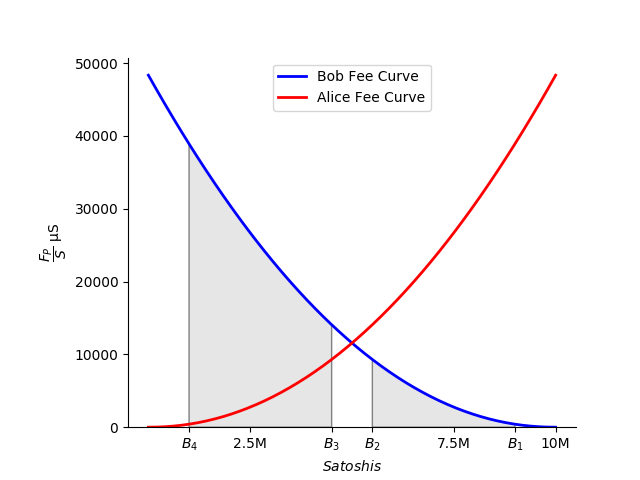
\includegraphics[width=10cm]{images/fee_scheme.png}
	\label{fig:xt_nodes}
\end{figure}
\newpage

From the cost function the fee may be retrieved by calculating the area under the graphs. Some deterministic way to round the fee to whole satoshis and some way to verify the function is formulated correctly must be defined. 

The fees for $P_1$, $P_2$ would be very different with this brackets method.

\[ F_{P_1} = F_{B} + \int_{B_1}^{B_2} f(x) dx = F_B + 13,502,153,930 \mu S \] 

\[ F_{P_2} = F_{B} + \int_{B_3}^{B_4} f(x) dx  = F_B + 88,984,850,361 \mu S \]
 
Here the fees are much larger for the payment that unbalances the channel than the payment that balances it. 

Brackets would incentivize payments to route in such a way to keep channels balanced which may lead to higher throughput. %I will most likely do a few simulations later this spring to validate this methods affect on the network.

This method has clearly some headaches accompanying it. It may be unnecessarily complex and would requires deterministic ways to calculate integrals over multiple systems. There might be better ways to solve this problem and there might be problems with this approach I'm unaware of. Anyway, some small tweaks in the protocol may lead to a much healthier network which may be worthy of exploration.\\

\textbf{John-John Markstedt}



    \printglossary[type=main]
   
  %  \chapter{Mirrors}

\begin{displayquote}
	\centering
	“Who controls the past controls the future.
	\\ Who controls the present controls the past.”
	\\ - George Orwell 
	
\end{displayquote}

\bibliography{mirror.bib}

	\end{appendices}

\end{document}
